\documentclass[a4paper]{article}
\usepackage[utf8]{inputenc}

\title{Error-correctie van QR-codes}
\author{Tjeu Kayim}
\date{16 december 2016}
\usepackage[T1]{fontenc}
\usepackage[scaled=0.85]{beramono}
%\usepackage{bold}
\usepackage{minted}
\usepackage{tikz}
\usepackage{subcaption}
%\usemintedstyle{tango}
\usepackage{amsmath}
\usepackage{breqn} % om lange polynomen automatisch te verdelen over verschillende regels
\usepackage{amssymb}
\usepackage{multirow}
\usepackage{wrapfig}
\usepackage{tabto}
%\usepackage{polynom}
\usepackage{fullpage}
\usepackage{pdflscape}
\usepackage[dutch]{babel}
\usepackage{graphicx}
\usepackage{incgraph}
\graphicspath{ {images/} }

\begin{document}
\newcommand*\xor{\mathbin{\oplus}}
\def\blockms#1{\begin{minipage}{\linewidth} \texttt{#1}\end{minipage}}
\def\boldms#1{\texttt{\textbf{#1}}}

\incgraph{Voorblad.pdf}


\maketitle
\tableofcontents
\newpage

\section{Inleiding}
Dit profielwerkstuk behandelt een toepassing van wiskunde voor digitale apparaten: methodes om informatie zo te coderen dat later eventuele fouten gecorrigeerd kunnen worden door wiskundige algoritmes. Het vakgebied van wiskundige error-correctie heet coderingstheorie. Deel één gaat over coderingstheorie in het algemeen, en behandelt ook de Hamming-code. In het tweede deel wordt uitgelegd hoe coderingstheorie een toepassing heeft in QR-codes. Het hele proces van het maken van QR-codes wordt behandeld, inclusief de nodige wiskunde. Daarnaast laat ik zien hoe het bouwen van een QR-code geprogrammeerd kan worden in de taal Python.

% *** verband alinea mist
Dit onderwerp sprak me aan omdat het een praktische toepassing is. Ik ben redelijk goed met wiskunde, maar vindt het pas echt interessant als het een duidelijke toepassing krijgt. Bij dit onderwerp kon ik ook nog programmeren, wat ik best leuk vindt om te doen. Ik heb me altijd al afgevraagd hoe zo'n QR-code nu echt werkt, dus toen ik op de site van de TU in Eindhoven las hoe coderingstheorie als profielwerkstukonderwerp werd aangeraden, dacht ik: Waarom combineer ik dat niet met elkaar, en ga ik uitzoeken hoe de error-correctie van QR-codes werkt? Het bleek een stuk ingewikkelder dan ik had gedacht, maar de wiskunde was te doen.

Tijdens het bestuderen van de wiskunde die nodig is voor QR-codes, viel het me op hoeveel wiskunde er is waar ik nog nooit van had gehoord. Toch speelt het allemaal een rol bij een QR-code. Het werd me duidelijk dat ik ergens een grens moest trekken hoe diep ik het onderwerp zou gaan onderzoeken. Ik heb daarom besloten om te stoppen bij de foutdetectie, en niet uit te werken hoe de ingewikkelde algoritmes werken die worden gebruikt om fouten in QR-codes te corrigeren.

Ik moest accepteren dat het in de digitale wereld waarin we leven onmogelijk is om alle techniek volledig te begrijpen. We maken vaak gebruik van erg complexe apparaten terwijl we niet precies weten hoe ze werken. Soms denken we te weten hoe iets werkt, maar blijkt het eigenlijk veel ingewikkelder te zijn. Of je denkt juist dat je nooit zal kunnen snappen hoe een bepaalde techniek werkt, en begint er dan ook niet aan.

Toch is het vaak nog goed te doen om een globaal beeld te krijgen van de werking van techniek en de details achterwege te laten. Ik zal daarom proberen een duidelijk overzicht te geven van de verschillende stappen voor het bouwen van een QR-code. Ik laat wel de nodige wiskunde zien, voor degene die QR-codes van het begin tot het einde willen begrijpen.

Omdat ik wil uitleggen hoe QR-codes werken heb ik de volgende hoofdvraag gekozen: Hoe wordt coderingstheorie toegepast in QR-codes? Ik heb gekozen voor deze hoofdvraag omdat ik zelf erg nieuwsgierig was naar de error-correctie van QR-codes, en het breed genoeg is om een werkstuk over te schrijven. Ik heb een aantal deelvragen om de coderingstheorie in te leiden:
\begin{itemize}
\item Wat is het nut van coderinstheorie en wat zijn de toepassingen?
\item Welke ontwikkelingen hebben binnen de coderingstheorie plaatsgevonden?
\item Hoe zijn de verschillende foutcorrigerende methodes te vergelijken?
\end{itemize}

Daarna wordt de deelvraag `Hoe werkt de Hamming-code?' beantwoord, als opstapje naar de Reed-Solomoncode. Vervolgens wordt aan de hand van vijf deelvragen de werking van QR-codes behandeld:
\begin{itemize}
\item Hoe werkt een QR-code?
\item Hoe wordt tekst omgezet naar bits?
\item Hoe werkt de Reed-Solomoncode, en hoe wordt die hier toegepast?
\item Hoe bouw je een QR-code?
\item Hoe werkt het decoderen?
\end{itemize}

Leuk dat je de moeite hebt genomen dit werkstuk te lezen. Wil je alleen een globaal beeld van de opbouw van een QR-code, kan je de pagina's vol code en wiskunde best overslaan. Maar wil je juist meer weten, kan je de wiskunde achter de RS-code verder uitzoeken. Of gebruik deze uitleg om zelf een QR-code-generator te programmeren.

Succes met lezen!

\section{Wat is coderingstheorie?}
\subsection{Wat is het nut van coderingstheorie en wat zijn de toepassingen?}
Bij elke overdracht van informatie kunnen fouten worden gemaakt. Als je met iemand praat, kan het zijn dat je de ander niet verstaat. Je zou een woord verkeerd kunnen uitspreken, of de ander verstaat het verkeerd. Als je een CD afspeelt, kan het het zijn dat de speler hapert doordat er krassen op de CD zitten. Als computers digitaal informatie versturen of ontvangen, kunnen er ook fouten optreden. Vaak ontstaan die fouten door ‘ruis’.

Ruis bestaat uit willekeurige variaties in een signaal. Die variaties hebben allerlei oorzaken, bij een radio ontstaat ruis bijvoorbeeld door alle kanalen die elkaar storen, of door kosmische straling. Hoe krachtiger het signaal is, hoe kleiner de kans is op fouten door ruis. Digitale signalen hebben minder last van ruis dan analoge, maar er blijft altijd een kleine kans op fouten.

Soms is er maar een heel zwak signaal, bijvoorbeeld bij de communicatie met een marsrover. Door de lage signaal-ruis verhouding is de kans op fouten dan erg groot. Voor dat soort situaties zijn er technieken bedacht om fouten te corrigeren.

Toepassingen van coderingstheorie vindt je ook in CD's, bij communicatie met satellieten of ruimtesondes, bij telefonie, bij Wifi en andere vormen van digitale communicatie.
\subsection{Welke ontwikkelingen hebben binnen de coderingstheorie plaatsgevonden?}
Toen in de 20e eeuw allerlei digitale apparaten werden uitgevonden, werd het soms nodig om fouten te detecteren. In 1951 werd een enkelvoudige pariteitscontrole gebruikt om informatie op tape op te slaan.

Dat werkt zo: De bits (enen en nullen) worden in groepen verdeeld, en van elke groep bepaal je de som van de bits. Is de som even, dan voeg je een \texttt{0} toe als pariteitsbit, en is de som oneven, dan voeg je een \texttt{1} toe. Als er dan één fout optreedt, klopt de pariteitsbit niet meer, en zo kun je achterhalen dat er iets verkeerd ging. Deze pariteitscontrole kan  niet meer dan één fout detecteren, en kan ook niet de fout corrigeren.

De simpelste manier om fouten, niet alleen te detecteren, maar ook te corrigeren, is het herhalen van elke bit. Dus de rij ‘\texttt{1 0 0 1}’ wordt bijvoorbeeld ‘\texttt{11111 00000 00000 11111}’. Fouten kunnen dan worden verbeterd door in elk groepje te tellen welke bits het meeste voorkomt. Ontvang je \texttt{10011}, is de kans het grootste dat er \texttt{11111} heeft gestaan. Deze methode maakt het bericht veel langer, en is dus helemaal niet efficiënt.

De wiskundige Claude Shannon onderzocht dit probleem. Hij gaf het wiskundige bewijs dat het mogelijk was om berichten te coderen op zo'n manier dat het aantal extra bits zo klein mogelijk wordt gehouden. Hiermee legde hij de basis van de coderingstheorie. Helaas bevatte zijn bewijs geen specifieke methodes voor efficiënte codes. Hij formuleerde de `wet van Shannon-Hartley' die ook wel bekend staat als Shannonlimiet.
Deze formule geeft het verband tussen de maximale hoeveelheid informatie die zonder fouten kan worden verzonden ($C$ in bits per seconde), de bandbreedte van het kanaal ($BW$) en de signaal-ruisverhouding ($S/N$).

$$C = BW \cdot \log_2(1+S/N)$$

Deze formule voorspelt dus hoever coderingstheorie kan gaan en wat het limiet is van de efficiëntie. Sindsdien komen nieuwe codes steeds dichter in de buurt van de Shannonlimiet, zoals Low-density parity-check codes, Polar codes en Turbocodes.

Richard Hamming bedacht als een van de eersten een efficiënte fout-corrigerende code. In de jaren 40 werkte hij met computers die hun input via ponskaarten kregen. De lezer van die ponskaarten was erg foutgevoelig, en daar wilde Hamming wat tegen doen. Hij bedacht een fout-corrigerende code die nu naar hem is vernoemd, de Hamming-code.

Rond die tijd werden ook de Golay codes, en de Reed-Muller code ontwikkeld. In de jaren 60 werden de BHC codes ontwikkeld, waaronder de Reed-Solomoncodes. Deze codes waren een grote verbetering in efficiëntie. In 1969 werd de Reed-Muller code toegepast voor communicatie met een Mariner-sone die naar Mars werd gestuurd.

Door de verdere reizen van ruimtesondes, zoals de Voyager en de Galileo missie, waren er codes nodig die kunnen werken bij extreem veel ruis. Het signaal wordt door de grote afstanden zo afgezwakt, dat het heel erg wordt verstoord.

Een oplossing was om verschillende codes tegelijk toe te passen. In 1993 werden Turbocodes voor het eerst beschreven door drie Franse wiskundigen. Door tweemaal te coderen met verschillende verbanden kunnen extra fouten worden gecorrigeerd. Zulke codes halen bijna de Shannonlimiet, en zijn dus erg efficiënt.

In 1996 werden Low-density parity-check codes (LDPC) herontdekt, die al in 1963 door Gallager waren ontwikkeld. In die tijd waren ze alleen erg onpraktisch vanwege de grote complexiteit, en werden ze vergeten. Maar computers zijn een stuk sneller geworden, en nu worden LDPC codes volop gebruikt, bijvoorbeeld bij Wifi.

\begin{figure}[!htbp]
\centering
\includegraphics[width=0.7\linewidth]{vergelijking3.png}
\caption[Spectrale efficiëntie uitgezet tegen capaciteit van verschillende fout-corrigerende codes]{Spectrale efficiëntie uitgezet tegen capaciteit van verschillende fout-corrigerende codes\footnotemark}
\label{fig:vergelijking}
\end{figure}
\footnotetext{Afbeelding uit `A Brief History of Coding Theory' door Matthieu Bloch}


\subsection{Hoe zijn de verschillende foutcorrigerende methodes te vergelijken?}
In Figuur \ref{fig:vergelijking} is te zien welke foutcorrigerende codes er allemaal zijn ontwikkeld. Dit overzicht is niet volledig, maar bevat de meestgebruikte codes. Bij het vergelijken moet met drie dingen rekening worden gehouden:

Ten eerste moet het natuurlijk niet te veel ruimte innemen. De efficiëntie van een code is te bepalen door de spectrale efficiëntie te berekenen. Bij elke foutcorrigerende code wordt er informatie toegevoegd, en wordt het bericht langer. Die extra informatie noemen we redundantie. Een efficiënte code moet dus met zo weinig mogelijk redundantie werken. De spectrale efficiëntie is gedefinieerd als het aantal informatieve bits dat per tijdseenheid wordt verzonden. Dat getal is hoger voor een code met minder redundantie. Codes hoog in de grafiek zijn dus efficiënter, omdat ze minder ruimte innemen.

Ook het aantal fouten dat kan worden gecorrigeerd verschilt. Dat kan worden uitgedrukt in de `power efficiency'. Een lagere power-efficiency betekent dat er meer fouten gecorrigeerd kunnen worden. In de grafiek staan links de codes met de beste error-correctie.

Als laatste is ook de rekenkracht van belang die nodig is bij het coderen. Vroeger was dit belangrijker dan nu, vanwege de trage computers. Maar doordat processoren veel sneller zijn geworden, kunnen nu zelfs smartphones gebruik maken van ingewikkelde codes. Nu weegt efficiëntie veel zwaarder dan de nodige rekenkracht. Voor 5G, de opvolger van 4G, wordt bijvoorbeeld overwogen om de Polar Code (PC) te gebruiken. Deze code haalt bijna de Shannonlimiet, maar vergt wel veel rekenkracht.

Voor elke toepassing kan weer een andere code beter aan je eisen voldoen. 
Wil je bijvoorbeeld een foutcorrigerende code gebruiken om bestanden te e-mailen, is er maar weinig ruis, en gaat het er vooral om dat de code niet te veel ruimte inneemt. Dan moet je een code kiezen die hoog in de grafiek staat, zoals de RS(255,223) code.

Maar ben je bijvoorbeeld een radiozender aan het bouwen, heb je juist veel meer aan een code links in de grafiek, omdat er veel ruis in het signaal zal komen. In dat geval zou je het best kunnen kiezen voor de LDPC-code of Turbocodes.

\subsection{Hoe werkt de Hamming-code?}
De Hamming-code is een eenvoudige foutcorrigerende code, het is efficiënt, maar makkelijk te begrijpen en zelfs te visualiseren. Daardoor is het een goede manier om te gaan begrijpen hoe coderingstheorie werkt.

De (7,4) Hamming-code kan voorgesteld worden door drie cirkels die elkaar overlappen. In elk gebied tussen de cirkels komt een bit, een \texttt{1} of een \texttt{0}. $d_0$ tot $d_3$ bevatten de te coderen informatie, en de pariteitsbits $p_0$, $p_1$ en $p_2$ worden toegevoegd als redundantie.

Stel we willen de letters `QR' coderen met de Hamming-code. Eerst moeten de letters worden omgezet naar bits met bijvoorbeeld UTF-8. De Q wordt \texttt{01010001} en de `R' \texttt{01010010}. Hoe dit omzetten precies werkt leg ik over twee hoofdstukken uit.
Na het omzetten naar bits verdelen we de bits in groepjes van vier.
\[\texttt{`QR' --> 0101000101010010 --> 0101 0001 0101 0010}\]
Elk groepje coderen we nu met de Hamming-code. Dat doen we met behulp van drie cirkels. Hieronder is te zien hoe de eerste vier bits in de cirkels worden geplaatst. Heb je dat gedaan, kan je de pariteitsbits bepalen. In elke cirkel moet een even aantal enen komen te staan. De bits die toegevoegd worden, moeten zo worden gekozen dat aan die voorwaarde wordt voldaan. Staan er dus twee enen in een cirkel, moet een \texttt{0} worden toegevoegd. Staan er drie enen, voeg je nog een \texttt{1} toe om het aantal even te maken.

%\begin{wrapfigure}[18]{r}{0.4\linewidth}
\begin{figure}[H]
\begin{subfigure}{.33\textwidth}
    \centering
    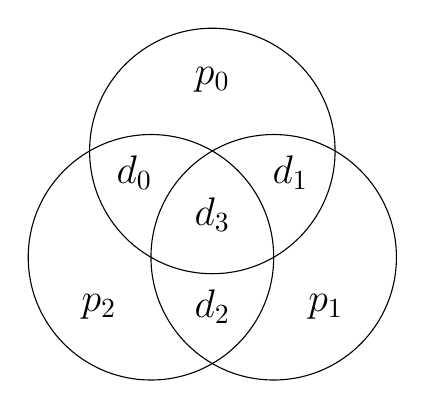
\begin{tikzpicture}[%
        scale = 0.9
    ]
      \draw (0,1) circle [radius=1.732];
      \draw (0.866,-.5) circle [radius=1.732];
      \draw (-0.866,-.5) circle [radius=1.732];
      \node (c) at (1.1,0.7) {\Large $d_1$};
      \node (c) at (-1.1,0.7) {\Large $d_0$};
      \node (c) at (0,.1) {\Large $d_3$};
      \node (c) at (0,-1.2) {\Large $d_2$};
      \node (c) at (0,2) {\Large $p_0$};
      \node (c) at (1.6,-1.2) {\Large $p_1$};
      \node (c) at (-1.6,-1.2) {\Large $p_2$};
    \end{tikzpicture}
    \caption*{Hamming-code}
\end{subfigure}
\begin{subfigure}{.33\textwidth}
    \centering
    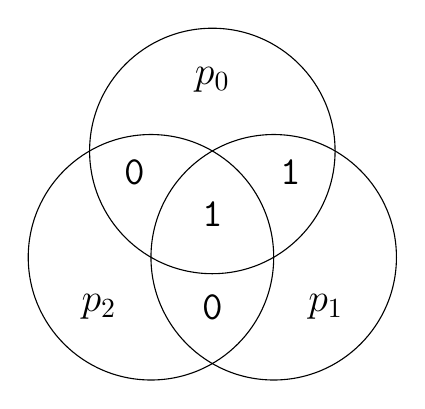
\begin{tikzpicture}[%
        scale = 0.9
    ]
      \draw (0,1) circle [radius=1.732];
      \draw (0.866,-.5) circle [radius=1.732];
      \draw (-0.866,-.5) circle [radius=1.732];
      \node (c) at (1.1,0.7) {\Large \texttt{1}};
      \node (c) at (-1.1,0.7) {\Large \texttt{0}};
      \node (c) at (0,.1) {\Large \texttt{1}};
      \node (c) at (0,-1.2) {\Large \texttt{0}};
      \node (c) at (0,2) {\Large $p_0$};
      \node (c) at (1.6,-1.2) {\Large $p_1$};
      \node (c) at (-1.6,-1.2) {\Large $p_2$};
    \end{tikzpicture}
    \caption*{\texttt{0101} invullen}
\end{subfigure}
\begin{subfigure}{.33\textwidth}
    \centering
    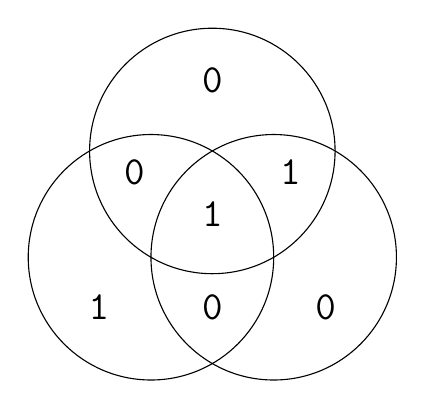
\begin{tikzpicture}[%
        scale = 0.9
    ]
      \draw (0,1) circle [radius=1.732];
      \draw (0.866,-.5) circle [radius=1.732];
      \draw (-0.866,-.5) circle [radius=1.732];
      \node (c) at (1.1,0.7) {\Large \texttt{1}};
      \node (c) at (-1.1,0.7) {\Large \texttt{0}};
      \node (c) at (0,.1) {\Large \texttt{1}};
      \node (c) at (0,-1.2) {\Large \texttt{0}};
      \node (c) at (0,2) {\Large \texttt{0}};
      \node (c) at (1.6,-1.2) {\Large \texttt{0}};
      \node (c) at (-1.6,-1.2) {\Large \texttt{1}};
    \end{tikzpicture}
    \caption*{pariteitsbits toegevoegd}
\end{subfigure}
\caption{(7,4) Hamming-code}
\end{figure}

Voeg nu de pariteitsbits toe aan de andere bits, en het bericht is gecodeerd:
\[\texttt{0101 001}\]

Wat heb je nu aan die drie extra bits? Als er nu fouten in het bericht komen, kunnen die worden verbeterd. Ontvang je bijvoorbeeld \texttt{1101001}, dan kom je erachter dat er iets mis is. Teken de bits maar in de cirkels, dan krijg je dit:
\definecolor{red}{RGB}{255, 30, 0}
\begin{figure}[H]
    \centering
    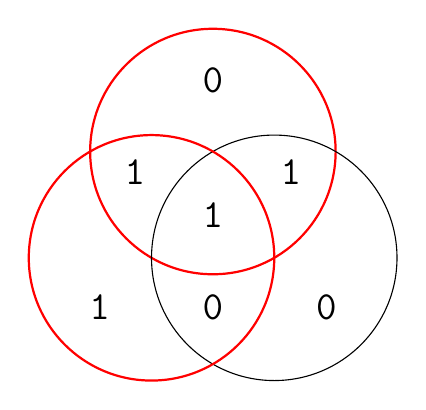
\begin{tikzpicture}[%
        scale = 0.9
    ]
      \draw [color=red, thick] (0,1) circle [radius=1.732];
      \draw (0.866,-.5) circle [radius=1.732];
      \draw [color=red, thick] (-0.866,-.5) circle [radius=1.732];
      \node (c) at (1.1,0.7) {\Large \texttt{1}};
      \node (c) at (-1.1,0.7) {\Large \bf \texttt{1}};
      \node (c) at (0,.1) {\Large \texttt{1}};
      \node (c) at (0,-1.2) {\Large \texttt{0}};
      \node (c) at (0,2) {\Large \texttt{0}};
      \node (c) at (1.6,-1.2) {\Large \texttt{0}};
      \node (c) at (-1.6,-1.2) {\Large \texttt{1}};
    \end{tikzpicture}
\end{figure}

In de rode cirkels zijn het aantal enen niet even. Er zit dus ergens een foutje. De positie van de fout is blijkbaar in de rode cirkels, maar buiten de zwarte. Er is maar een plaats die daaraan voldoet: linksboven. De \texttt{1} die daar staat had dus een \texttt{0} moeten zijn.

De Hamming code is redelijk eenvoudig te programmeren. Ik heb hieronder in Python een programma geschreven dat een bericht kan coderen.

\begin{minted}[fontsize=\small]{python}
def to_utf8(msg):
    ''' Zet tekst om naar bits met UTF-8 '''
    msg = bytes(msg, "utf8")
    return ''.join(["{0:08b}".format(x) for x in msg])

def encode(msg):
    ''' Codeer met de (7,4) Hamming code '''
    # Zet om naar bits
    msg = to_utf8(msg)
    # Splits de bits in groepjes van 4
    msg = [msg[i:4 + i] for i in range(0, len(msg), 4)]
    # Funtie om de pariteit te berekenen
    def p (*args):
        pariteit = 0
        for x in args:
            pariteit ^= int(bits[x])
        return str(pariteit)
    # Voeg aan elk groepje de pariteitbits toe
    msg_out = ''
    for bits in msg:
        msg_out += bits + p(0,1,3) + p(1,2,3) + p(0,2,3)
    return msg_out
\end{minted}

Vond je dit hoofdstuk interessant, probeer dan zelf dit gecodeerde bericht te decoderen met behulp van Figuur \ref{fig:unicode}. Maar let op, er zitten wel fouten in.

\[\texttt{0110110 0110100 0110101 1101111 0101010 0101001}\]
\[\texttt{0111010 0100010 0100101 1010110 1110101 0100001}\]

Dit voorbeeld maakt duidelijk hoe de Hamming-code werkt. QR-codes maken gebruik van een moeilijkere code, die wel efficiënter is, namelijk de Reed-Solomoncode. Toch blijft het idee hetzelfde: je voegt bits toe die aan een bepaalde voorwaarde moeten voldoen, en later kan je daardoor fouten corrigeren.
\section{Hoe wordt coderingstheorie toegepast in QR-codes?}

\subsection{Hoe werkt een QR-code?}
\begin{figure}[htbp]
    \centering
    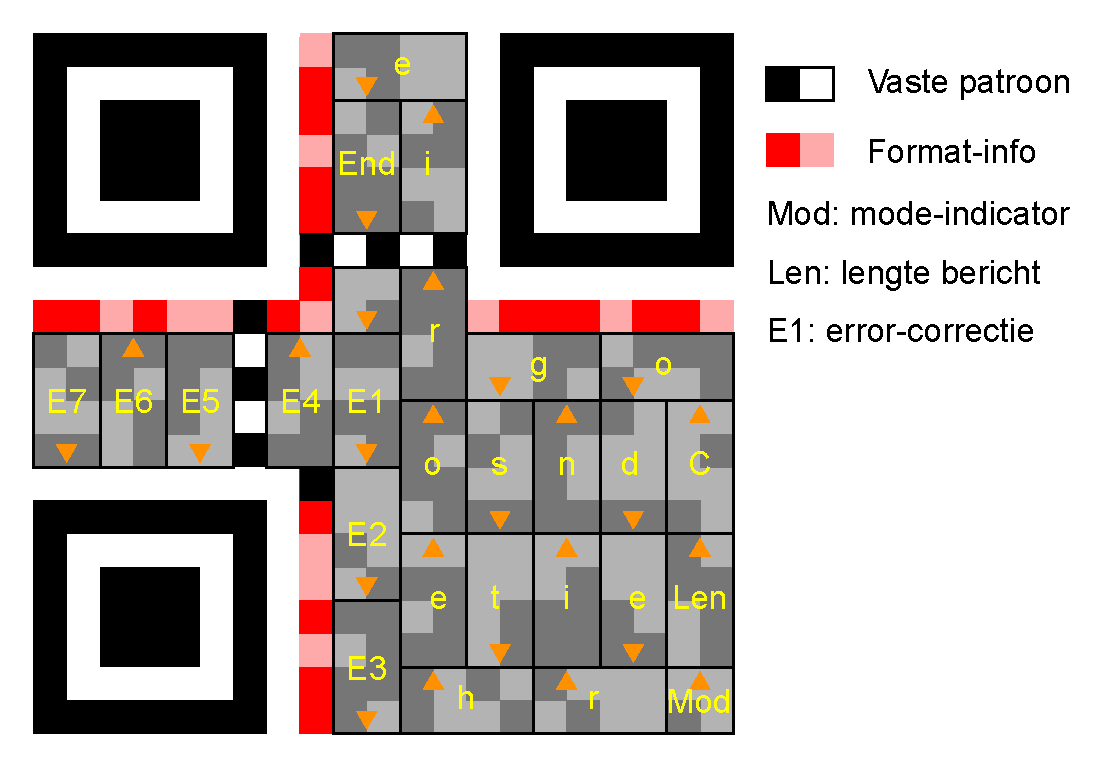
\includegraphics[width=0.6\textwidth]{plaatsing-letters.pdf}
    \caption[Plaatsing letters in een QR-code]{Plaatsing letters in een QR-code\footnotemark}
    \label{fig:plaatsing}
\end{figure}
\footnotetext{Afbeelding zelf aangepast en vertaald, origineel te vinden op \url{https://commons.wikimedia.org/w/index.php?curid=16981996}}

Een QR-code is een twee-dimensionale streepjescode: een zwart wit geblokt vierkantje, dat je kan scannen met je smartphone. Qr-codes worden gebruikt om informatie vast te leggen in een afbeelding, die makkelijk door een elektronisch apparaat gescand kan worden. De QR-code is bedacht in Japan, en was ontworpen om onderdelen te labelen in de auto-industrie. Maar nu hebben QR-codes veel andere toepassingen gekregen, zoals bij smartphones. De bekendste toepassing is een URL: een link naar een website of applicatie. Als de code door een smartphone wordt gescand, herkent de software de QR-code, decodeert de informatie en opent de URL in een webbrowser.

Het maken van QR-codes wordt meestal door computers of smartphones gedaan, omdat er veel gerekend moet worden met andere rekenregels. Om een goede uitleg te geven, laat ik zien hoe je stap voor stap een QR-code kan maken met daarin de tekst `Coderingstheorie'. Je zult zien dat het veel werk is om met de hand een QR-code te bouwen, terwijl we de kleinste grootte gebruiken.

Er zijn namelijk verschillende groottes qr-codes, en verschillende error-correctie levels. We gebruiken de e.c-level met de minste redundantie, zodat we het nog met de hand kunnen berekenen. Het woord `Coderingstheorie' past dan nog net in de kleinste grootte: Versie 1.

Het moeilijkste onderdeel zit in het inbouwen van de Reed-Solomoncode (RS-code) als foutdetectie. Deze code is erg efficiënt, maar er is wel veel wiskunde voor nodig.

Voordat we het bericht kunnen coderen met de RS-code, moet het bericht eerst worden omgezet in bits. Dat gebeurt in vier stappen:
\begin{itemize}
    \item Het bericht wordt met UTF-8 omgezet naar bytes.
    \item Aan de bits wordt informatie toegevoegd over de `soort' data.
    \item Er wordt toegevoegd hoeveel letters het bericht bevat.
    \item De bits worden aangevuld totdat de maximale lengte is bereikt.
\end{itemize}

\begin{figure}[!htbp]
\centering
\includegraphics[width=0.3\linewidth]{hex-dec-bin-table2.png}
\caption{Hexadecimaal, Decimaal en Binair}
\label{fig:bin}
\end{figure}

\subsection{Hoe wordt tekst omgezet naar bits?}
\subsubsection{Bits, bytes \& binair}
Computers rekenen met bits: enen en nullen. Omdat QR-codes door computers worden gemaakt en gelezen, zul je vaak lezen over bits, bytes en binaire bewerkingen, zoals Exclusive OR. Een bit is \texttt{1} of \texttt{0}. Een byte is een groepje van acht bits.

Bits kunnen gezien worden als getallen, maar er kunnen ook speciale bewerkingen mee worden gedaan. In principe kan je met bits alle `normale' sommen oplossen. Je kunt bits onder elkaar zetten om ze op te tellen of te vermenigvuldigen, net als met normale getallen. Alleen hoef je maar twee tafels uit je hooft te kennen voor het vermenigvuldigen. Dat betekent wel dat een vermenigvuldiging met bits veel meer tussenstappen telt.

Figuur \ref{fig:bin} laat zien hoe bits om te rekenen zijn naar decimale of hexadecimale getallen. ‘Dec’ staat voor decimaal, de normale schrijfwijze van getallen met tien cijfers. Daarnaast staat de Hexadecimale notatie: een talstelsel waarbij niet met tien cijfers, maar met zestien cijfers wordt geteld. De cijfers 0 t/m 9 worden uitgebreid met 'A' (10) t/m 'F' (15). De hexadecimale notatie wordt vaak gebruikt om binaire getallen kort te schrijven. Computers werken met bytes, acht bits, en die zijn met precies twee hexadecimale cijfers te schrijven. 

Om bits naar decimale getallen om te rekenen maak je gebruik van machten van 2. Kijk eerst eens hoe normale getallen te schrijven zijn met machten van 10:

$$1234 = 1\cdot10^3 + 2\cdot10^2 + 3\cdot10^1 + 4$$

En nu doen we dat met bits:

$$\texttt{1 0 1 1 0} = 1\cdot2^4 + 0\cdot2^3 + 1\cdot2^2 + 1\cdot2^1 + 0$$
$$= 16 + 4 + 2 = 22$$

Dus het getal 22 is binair \texttt{10110}.

\subsubsection{UTF-8}
\begin{figure}[!htbp]
\centering
\includegraphics[width=0.5\linewidth]{unicode.png}
\caption{UTF-8}
\label{fig:unicode}
\end{figure}
Om te beginnen moet de boodschap omgezet worden van letters naar bytes, we maken daarbij gebruik van UTF-8. In Figuur \ref{fig:unicode} is een deel van de tabel te zien om letters te coderen.

We coderen dus het woord ‘Coderingstheorie’ met UTF-8 naar hexadecimale getallen:

\texttt{
\begin{tabular}{llllllllllllllll}
C&o&d&e&r&i&n&g&s&t&h&e&o&r&i&e\\
43&6F&64&65&72&69&6E&67&73&74&68&65&6F&72&69&65\\
\end{tabular}
}

Dan zetten we dat om naar binair:\\\\
\blockms{01000011 011011110 11001000 11001010 11100100 11010010 11011100 11001110 11100110 11101000 11010000 11001010 11011110 11100100 110100101 100101\\}
Deze stappen worden ook uitgevoerd als je een Word document opslaat, of als je een Whatsapp berichtje verstuurd.
\subsubsection{Mode-indicator \& Character-count}
Nu voegen we wat informatie toe die nodig is bij het scannen van de QR-code. We moeten duidelijk maken dat we UTF-8 hebben gebruikt door een ‘mode-indicator’ toe te voegen: dat is in dit geval \boldms{0100}. Daarna komt nog een ‘character-count’: het aantal letters in het bericht. In dit geval zijn dat er 16, binair geschreven \boldms{00010000}.\\\\
\blockms{\textbf{0100 00010000} 01000011 01101111 01100100 01100101 01110010 01101001 01101110 01100111 01110011 01110100 01101000 01100101 01101111 01110010 01101001 01100101\\}

Daarna wordt alles in bytes verdeeld (groepjes van acht bits) en vullen we de laatste byte verder op met nullen:\\\\
\blockms{01000001 00000100 00110110 11110110 01000110 01010111 00100110 10010110 11100110 01110111 00110111 01000110 10000110 01010110 11110111 00100110 10010110 0101\textbf{0000}\\}

Er passen 19 bytes in een versie 1 QR-code, en we zitten nu op 18. De rest moet worden opgevuld met het herhalen van de bytes \boldms{11101100} en  \boldms{00010001} totdat de maximale capaciteit is bereikt. In dit geval al na het toevoegen van één byte.\\\\
\blockms{01000001 00000100 00110110 11110110 01000110 01010111 00100110 10010110 11100110 01110111 00110111 01000110 10000110 01010110 11110111 00100110 10010110 01010000 \textbf{11101100}\\}
Dat zetten we dit om naar de hexadecimale notatie:\\\\
\blockms{41 04 36 F6 46 57 26 96 E6 77 37 46 86 56 F7 26 96 50 EC\\}

Zo wordt het te coderen bericht dus omgezet naar bytes. In grotere QR-codes worden deze bytes nog gesplitst in meerdere blokken, waarvan allemaal afzonderlijk error-correctie-bytes worden berekent. Hierover later meer.
Ik heb voor het omzetten naar bytes een programma geschreven in de programmeertaal Python:
\begin{minted}[fontsize=\small]{python}
# (alles waarvoor een hekje staat is uitleg)
# Definiëer een functie die tekst codeert met uft-8
def qr_encode_to_utf8(tekst,n):
    # zet tekst om in utf-8
    tekst = bytes(tekst, "utf8")
    # zet om naar bytes
    bits = ''.join(["{0:08b}".format(x) for x in tekst])
    # voeg de `mode indicator' en het aantal tekens toe 
    bits = '0100' + "{0:08b}".format(len(tekst)) + bits
    # voeg nullen toe totdat een veelvoud van 8 is bereikt
    # of de maximale lengte is bereikt
    while len(bits) % 8 and len(bits) != n*8:
        bits += '0'
    # past het wel?
    if len(bits) > n*8:
        print('Het te coderen bericht is te groot voor deze versie')
        return
    # herhaal 11101100 en 00010001 totdat de maximale lengte is bereikt
    i = 0
    while len(bits) != n*8:
        if i%2: bits += '00010001'
        else: bits += '11101100'
        i += 1
    return bits
\end{minted}
\subsection{Hoe werkt de Reed-Solomoncode, en hoe wordt die hier toegepast?}
De Reed Solomoncode (RS-code) is een fout-corrigerende techniek en valt onder de BCH-codes. Het wordt bijvoorbeeld gebruikt bij error-correctie van DVD's en QR-codes. Door redundantie toe te voegen, kan een aantal fouten worden gecorrigeerd, net als bij de Hamming-code. Voor betere foutcorrectie is meer opslagruimte nodig door de extra redundantie. Maar de RS-code is daarin wel erg efficiënt, en er kunnen namelijk relatief veel fouten worden gecorigeerd met weinig redundantie. \par
De komende uitleg bevat veel ingewikkelde wiskunde, maar ik zal proberen duidelijk te maken waarvoor elk stukje wiskunde nuttig is. Ik zal ook laten zien hoe ik de wiskunde heb geïmplementeerd in een programma, geschreven in Python.

\subsubsection{Galoisveld}
De berekeningen bij de RS-code werken met polynomen in een $2^8$ Galoisveld. Dat is een lichaam met een eindig aantal elementen, in dit geval 0 tot en met 255. Dat zijn 256 elementen (0 telt ook mee), en zo'n Galoisveld wordt genoteerd als GF(256) of $\mathbb{F}_{256}$. Omdat de verzameling getallen eindig is, gelden er andere bewerkingen.\par
Het voordeel van dit Galoisveld is dat alle getallen precies in één byte byte passen, en dat is voor computers erg handig. Computers kunnen veel sneller en efficiënter werken als ze in een Galoisveld rekenen. Voor mensen rekent het helaas een stuk lastiger.

Een wiskundig lichaam maakt het dus mogelijk om te rekenen met een begrensd aantal getallen, maar daar zijn wel speciale rekenregels voor nodig. Want de bewerkingen optellen, aftrekken, vermenigvuldigen en delen moeten allemaal gesloten zijn. De uitkomsten moeten dus binnen het lichaam blijven.
\subsubsection{Optellen}
Optellen en aftrekken staat in dit Galoisveld gelijk aan de bewerking Exlusive OR (XOR). Dat is een binaire logische poort waarbij de output 1 is als de input één 1 bevat, anders is de output 0. De wiskundige notatie van XOR is $\xor$, en in veel programmeertalen wordt het genoteerd als een accent circonflexe: ^. Deze logische poort werkt zo:
$$0\xor0=0$$
$$1\xor1=0$$
$$1\xor0=1$$
$$0\xor1=1$$
Dit lijkt op optellen modulo 2:
$$0+0=0\mod{2}$$
$$1+1=0\mod{2}$$
$$1+0=1\mod{2}$$
$$0+1=1\mod{2}$$
Het optellen werkt met bits, dus moet je de getallen die je wilt optellen eerst omrekenen naar binaire getallen. Daarna zet je de getallen onder elkaar, en bereken je de som per bit. Om bijvoorbeeld $197 \xor 99$ te bereken doe je het volgende:
$$197 = 1\cdot2^7 + 1\cdot2^6 + 0\cdot2^5 + 0\cdot2^4 + 0\cdot2^3+ 1\cdot2^2 + 0\cdot2^1 + 1\cdot2^0$$
$$99 = 0\cdot2^7 + 1\cdot2^6 + 1\cdot2^5 + 0\cdot2^4 + 0\cdot2^3+ 0\cdot2^2 + 1\cdot2^1 + 1\cdot2^0$$
\\\blockms{\noindent
1 1 0 0 0 1 0 1 (197)\\
0 1 1 0 0 0 1 1 (99)\\
--------------------------- XOR\\
1 0 1 0 0 1 1 0\\
}
Dan rekenen we \texttt{10100110} weer om naar decimaal: $2^7+2^5+2^2+2^1=166$. Dus $197 \xor 99 = 166$.
\subsubsection{Vermenigvuldigen}
Vermenigvuldigen gaat met de rekenregel $2^a+2^b=2^{a+b}$. Alle coëfficiënten van de polynomen moeten dan dus geschreven worden als machten van twee: $2^n$, waarbij $n \in [0,255\rangle$. Maar alle getallen moeten wel in het Galoisveld $\mathbb{F}_{256}$ blijven. Tot $n = 7$ gaat dat goed:

$$2^0=1$$
$$2^1=2$$
$$2^2=4$$
$$2^3=8$$
$$2^4=16$$
$$2^5=32$$
$$2^6=64$$
$$2^7=128$$

Maar $2^8$ is te groot voor $\mathbb{F}_{256}$, en dan moeten het getal byte-wise modulo \texttt{100011101} genomen worden: er moet 258 vanaf getrokken worden, zoals is vastgesteld in de QR-code specificaties. Dus elke bit van $2^8$ (binair \texttt{100000000}) moet met 285 (binair \texttt{100011101}) worden geXORed.
\footnote{ISO/IEC 18004:2005 blz. 42}
285 is een irreducibele polynoom van de achtste graad. Het is niet te schrijven als het product van kleinere polynomen, en wordt ook wel een `priempolynoom' genoemd.\\\\
\blockms{100000000 (256)\\
100011101 (285)\\
--------------- XOR\\
000011101 (29)
}
\\\\
Nu kunnen we verder met de machten van 2.
$$2^8 = 29$$
$$2^9 = 2\cdot2^8 = 2\cdot29 = 58$$
$$2^{10} = 2^9 \cdot 2 = 58 \cdot 2 = 116$$

Zo kunnen we doorgaan tot $2^{254}$. Als dan bij het rekenen exponenten groter uitkomen dan 255, bijvoorbeeld bij $2^{250}+2^{10}=2^{260}$, dan moet de exponent modulo 255 genomen worden: $2^{260}=2^{260 \mod{255}}=2^5$. Met deze methode zijn alle getallen in $\mathbb{F}_{256}$ te schrijven als $2^n$, waarbij $n \in [0,255\rangle$.

Er is één uitzondering: 0, want $\log{0}$ bestaat niet. Maar dat is geen probleem, want vermenigvuldigen met 0 geeft altijd 0.

Voor het genereren van een tabel voor de exponenten en logaritmes heb ik functie geprogrammeerd. Ik heb er veel uitleg bijgeschreven om duidelijk te maken wat het programma doet.
\begin{minted}[fontsize=\small,mathescape]{python}
# Maak een lege tabel aan voor de exponenten van 2 in het Galoisveld (gf)
gf_exp = []
# en een tabel voor de logaritmes met 256 plaatsen
# (de eerste plaats wordt niet gebruikt, want log 0 bestaat niet)
gf_log = [0] * 256
# Deze functie vult de tabel, waarbij als argument de priempolynnoom moet worden gegeven
def tabel_exponenten(priem_polynoom):
    global gf_exp, gf_log
    x = 1 
    # $2^i = x$; i [0,255>
    for i in range(0,255):
        # voeg `x' ($=2^i$) toe aan de tabel voor exponenten
        gf_exp.append(x)
        # en voeg `i' toe aan de tabel voor logaritmes
        gf_log[x] = i
        # voor i+1 wordt x twee maal zo groot
        x = x*2
        # is x groter dan 255, XOR x dan met de priempolynoom
        # (XOR wordt genoteerd als ^)
        if x>255: x = x ^ priem_polynoom
# Maak een tabel met de priempolynoom 285
tabel_exponenten(285)
# De tabel wordt als volgt gebruikt
gf_exp[3] # = $2^3 = 8$
gf_log[8] # = $2\log{8} = 3$
\end{minted}

Vermenigvuldigen kan nu zo: $x\cdot y = \alpha^{^\alpha\!\log{x}+^\alpha\!\log{y} \mod 255}$
\begin{minted}[fontsize=\small,mathescape]{python}
# Vermenigvuldigen met de regel $2^a \cdot 2^b = 2^{a+b}$
# Definiëer een functie om de argumenten x en y te vermenigvuldigen.
def gf_mul(x,y):
    # Vermenigvuldigen met 0 geeft 0
    if x==0 or y==0:
        return 0
    # modulo wordt geschreven als %
    return gf_exp[(gf_log[x]+gf_log[y]) % 255]
\end{minted}
\subsubsection{Generatorpolynoom}

Voor coderen in de Reed-Solomoncode (RS-code) is een generatorpolynoom nodig: de polynoom waardoor straks gedeeld gaat worden. De rest bij die deling vormt de redundantie van de RS-code. Door de deling met deze polynoom ontstaat er een speciale wiskundige `verhouding' tussen het bericht en de redundantie, vergelijkbaar met de voorwaarden in de cirkels van de Hamming-Code. Die voorwaarden zijn nodig zodat er uiteindelijk eventuele fouten gecorrigeerd kunnen worden.

De generatorpolynoom voor de Reed-Solomoncode is als volgt gedefinieerd:
$$g_n(x)=\prod\limits_{i=0}^{n-1} x-\alpha^i = (x-\alpha^0)(x-\alpha^1)(x-\alpha^2) ... (x-\alpha^{n-1})$$

Waarbij $n$ het aantal fout-corrigerende codewoorden is dat moet worden gegenereerd. Bij het coderen van het woord `Coderingstheorie' is $n$ gelijk aan 22. Om verwarring met normaal machtsverheffen te voorkomen, is afgesproken om $2^n$ als $\alpha^n$ geschreven. Vanaf dit hoofdstuk zal ik die notatie gebruiken.

Om de haakjes van de generatorpolynoom weg te werken, moet rekening worden gehouden met de rekenregels van het eindige lichaam waarin we werken. Optellen en aftrekken word gedaan met Exclusive OR en vermenigvuldigen van $\alpha^b$ en $\alpha^c$ geeft $\alpha^{b+c}$. De notatie met machten zal dus een aantal keer omgerekend moeten worden naar bits, en andersom. Ik zal een beginnen met het berekenen van een generatorpolynoom voor twee error-correctie codewoorden.
$$g_2(x)=$$
$$(\alpha^0x - \alpha^0) \cdot (\alpha^0x - \alpha^1)=$$
$$(\alpha^0x^1 \cdot \alpha^0x^1) + (\alpha^0x^0 \cdot \alpha^0x^1) + (\alpha^0x^1 \cdot \alpha^1x^0) + (\alpha^0x^0 \cdot \alpha^1x^0)$$
Bij vermenigvuldigen de exponenten optellen:
$$(\alpha^{0+0}x^{1+1}) + (\alpha^{0+0}x^{0+1}) + (\alpha^{0+1}x^{1+0}) + (\alpha^{0+1}x^{0+0})=$$
$$\alpha^0x^2 + \alpha^0x^1 + \alpha^1x^1 + \alpha^1x^0=$$
$$\alpha^0x^2 + (\alpha^0+\alpha^1)x^1 + \alpha^1x^0$$
Optellen wordt gedaan met Exclusive OR.
$$x^2 + (1\xor2)x^1 + 2x^0$$
\blockms{01 (1)\\
10 (2)\\
------ XOR\\
11 (3)
}
$$x^2 + 3x^1 + 2x^0$$
Dan omrekenen naar de notatie met machten van alpha.
$$\alpha^0x^2 + \alpha^{25}x^1 + \alpha^1x^0$$
Dit is dus de generatorpolynoom voor twee codewoorden. Vermenigvuldigen we dat met $(x-\alpha^2)$, dan krijgen we $g_3(x)$.
$$g_3(x)=$$
$$(\alpha^0x^2 + \alpha^{25}x^1 + \alpha^1x^0) \cdot (\alpha^0x^1 + \alpha^2x^0)=$$
$$\alpha^0x^2 \cdot \alpha^0x^1 + \alpha^{25}x^1 \cdot \alpha^0x^1 + \alpha^1x^0 \cdot \alpha^0x^1 + \alpha^0x^2 \cdot \alpha^2x^0 + \alpha^25x^1 \cdot \alpha^2x^0 + \alpha^1x^0 \cdot \alpha^2x^0=$$
$$\alpha^{0+0}x^{2+1} + \alpha^{25+0}x^{1+1} + \alpha^{1+0}x^{0+1} + \alpha^{0+2}x^{2+0} + \alpha^{25+2}x^{1+0} + \alpha^{1+2}x^{0+0}=$$
$$\alpha^0x^3 + \alpha^{25}x^2 + \alpha^1x^1 + \alpha^2x^2 + \alpha^{27}x^1 + \alpha^3x^0=$$
$$\alpha^0x^3 + (\alpha^{25} \xor \alpha^2)x^2 + (\alpha^1 \xor \alpha^{27})x^1 + \alpha^3x^0=$$
$$\alpha^0x^3 + (3 \xor 4)x^2 + (2 \xor 12)x^1 + \alpha^3x^0=$$
\\
\blockms{011 (3)\\
100 (4)\\
--------- XOR\\
111 (7)\\
}
\blockms{1100 (12)\\
0010 (2)\\
--------- XOR\\
1110 (14)\\
}
$$\alpha^0x^3 + 7x^2 + 14x^1 + \alpha^3x^0=$$
$$\alpha^0x^3 + \alpha^{198}x^2 + \alpha^{199}x^1 + \alpha^3x^0$$
Ga zo verder tot $g_7(x)$:
$$g_4(x)=\alpha^{0}x^{4}+\alpha^{75}x^{3}+\alpha^{249}x^{2}+\alpha^{78}x+\alpha^{6}$$

$$g_5(x)=\alpha^{0}x^{5}+\alpha^{113}x^{4}+\alpha^{164}x^{3}+\alpha^{166}x^{2}+\alpha^{119}x+\alpha^{10}$$

$$g_6(x)=\alpha^{0}x^{6}+\alpha^{166}x^{5}+\alpha^{0}x^{4}+\alpha^{134}x^{3}+\alpha^{5}x^{2}+\alpha^{176}x+\alpha^{15}$$

$$g_7(x)=\alpha^{0}x^{7}+\alpha^{87}x^{6}+\alpha^{229}x^{5}+\alpha^{146}x^{4}+\alpha^{149}x^{3}+\alpha^{238}x^{2}+\alpha^{102}x+\alpha^{21}$$

Na deze bladzijdes wiskunde, weer wat programmeren. Om het woord `Coderingstheorie' te coderen hadden we $g_7(x)$ nodig. Om dit allemaal met de hand te doen, is erg langdradig, foutgevoelig en verschrikkelijk veel werk. Daarom heb ik het maken van een generatorpolynoom ook aan het programma toevoegen.

Eerst moet gedefinieerd worden hoe polynomen vermenigvuldigd  worden, en dan kan een functie gedefiniëerd worden om $g_n(x)$ te bereken.

\begin{minted}[fontsize=\small]{python}
# Polynomen vermenigvuldigen in een Galoisveld
# polynomen worden geschreven als een 'list' met coöficiënten
# x^2 + 3x - 6 => [1,3,-6]
def gf_poly_mul(p,q):
    # r(x) = p(x) * q(x)
    # de lengte van r(x) is gelijk aan de som van de lengtes van p(x) en q(x) min 1
    r = [0] * (len(p)+len(q)-1)
    for j in range(0, len(q)):
        for i in range(0, len(p)):
        	# Voor elke term in p(x), ga alle termen in q(x) af 
            # en tel het product van de te termen uit p(x) en q(x)
            # op bij de term van r(x), waarvan de exponent de som
            # is van de exponenten in de vermenigvuldigde termen
            # '^=' betekent: XOR dit met...
            r[i+j] ^= gf_mul(p[i], q[j])
            # Dit is zo'n voorbeeld waarbij de code een stuk simpeler is
            # dan de Nederlandse `uitleg'
    return r
\end{minted}
\begin{minted}[fontsize=\small]{python}
# Maak een Reed-Solomon (rs) generatorpolynoom
# voor een bepaald aantal error-correctie codewoorden (n)
def rs_generator_poly(n):
    # g(x)=1
    g = [1]
    # g(x)=1*(x-alpha^0)(x-alpha^1) ... (x-alpha^(n-1))
    for i in range(0,n):
        g = gf_poly_mul(g, [1, gf_exp[i]])
    return g
\end{minted}
\subsubsection{Synthetic Division}
In de volgende stap moeten de berichtpolynomen allebei gedeeld worden door de generatorpolynoom. Hiervoor gebruiken we de techniek `synthetische deling' of `extended synthetic division': een alternatief voor de staartdeling. Ik zal een korte uitleg geven. Stel je wilt deze deling oplossen:
$$\frac{
3x^4+200x^3+144x^2+250x+96
}{
1x^2 + 3x^1 + 2
}$$

Dat kan met een normale staartdeling voor polynomen, houdt er alleen rekening mee dat vermenigvuldigen met de alphanotatie moet, en aftrekken met Exclusive OR.
\[
\renewcommand\arraystretch{1.2}
\begin{array}{rrrrrrrr}
x^2+3x+2\text{ /} & 3x^4 & 200x^3 & 144x^2 & 250x & 96 & \text{\textbackslash} & 3x^2+205x+220\\
&3x^4 & 5x^3 & 6x^2 & \multicolumn{1}{l}{\xor}\\\cline{2-4}
&&205x^3 & 150x^2 & 250x\\
&&205x^3 & 74x^2 & 135x & \multicolumn{1}{l}{\xor} \\\cline{3-5}
&&&220x^2 & 125x & 96\\
&&&220x^2 & 121x & 165 & \multicolumn{1}{l}{\xor} \\\cline{4-6}
&&&&4x & 197
\end{array}
\]

Deze deling kan ook gedaan worden met de `Extended Synthetic division'. Deze methode werkt alleen als de eerste coëfficiënt van de noemer gelijk is aan één. Bij de generatorpolynomen, waardoor uiteindelijk gedeeld moet worden, is dat altijd het geval.

Eerst schrijf je de coëfficiënten op van de teller, beginnend bij de grootste exponent van $x$. De coëfficiënten van de noemer schrijf je in een schuine lijn naar boven op, behalve de eerste:
\[\begin{array}{rr|rrrrr}
&&3&200&144&250&96\\
&2\\
3&&
\end{array}\]

Daarna teken je onderaan een horizontale lijn, en breng je de het eerste getal bovenaan naar beneden:
\[\begin{array}{rr|rrrrr}
&&3&200&144&250&96\\
&2\\
3&&\\\cline{3-7}
&&3
\end{array}\]

Je vermenigvuldigt de drie met de coëfficiënten van de noemer. En schrijft de producten diagonaal op. In dit Galoisveld geld $3\cdot3=5$ en $3\cdot2=6$.
\[\begin{array}{rr|rrrrr}
&&3&200&144&250&96\\
&2&&&6\\
3&&&5\\\cline{3-7}
&&3
\end{array}\]

Dan bereken je de som in de volgende kolom en schrijft die onderaan op. Optellen werkt met Exlusive OR, en in dit geval komt er toevallig hetzelfde uit als bij normaal rekenen.
\[\begin{array}{rr|rrrrr}
&&3&200&144&250&96\\
&2&&&6\\
3&&&5\\\cline{3-7}
&&3&205
\end{array}\]

Het product van 205 met 3 en 2 schrijf je weer diagonaal op.
\[\begin{array}{rr|rrrrr}
&&3&200&144&250&96\\
&2&&&6&135\\
3&&&5&74\\\cline{3-7}
&&3&205
\end{array}\]

Herhaal deze stapen totdat de diagonaal niet meer zou passen. En schrijf de som van de laatste kolommen eronder.
\[\begin{array}{rr|rrrrr}
&&3&200&144&250&96\\
&2&&&6&135&165\\
3&&&5&74&122\\\cline{3-7}
&&3&205&220&4&197
\end{array}\]

De onderste regel zijn het quotiënt en de rest. Zet een streepje in de onderste regel zodat het aantal getallen rechts van het streepje gelijk is aan het aantal getallen links van de verticale lijn. Het streepje scheidt nu het quotiënt en de rest van elkaar.
\[\begin{array}{rr|rrrrr}
&&3&200&144&250&96\\
&2&&&6&135&165\\
3&&&5&74&122\\\cline{3-7}
&&3&205&\multicolumn{1}{r|}{220}&4&197
\end{array}\]
$$\frac{
3x^4+200x^3+144x^2+250x+96
}{
1x^2 + 3x^1 + 2
} = 3x^2 + 205x^1 + 220 + \frac{4x+197}{1x^2 + 3x^1 + 2}
$$

Deze methode is een stuk systematischer dan de staartdeling, en daardoor makkelijker te programmeren.
\begin{minted}[fontsize=\small]{python}
def poly_div(self,teller, noemer):
    '''Synthethic Division (Synthetische Deling)'''
    output = list(teller)
    # Voor alle diagonalen die passen
    for i in range(0, len(teller) - (len(noemer)-1)):
        # stop als de factor nul is, want log(0) bestaat niet
        if output[i] != 0:
            # de eerste coöficiënt van de noemer wordt overgeslagen
            for j in range(1, len(noemer)):
                 # stop als de factor nul is
                if noemer[j] != 0:
                    # vermenigvuldig en tel op (XOR) bij het getal onderaan de kolom
                    output[i+j] ^= self.mul(noemer[j], output[i])
    # bepaal de positie van van het verticale streepje
    # tussen het quotiënt en de teller
    streepje = -(len(noemer)-1)
    # en geef als resultaat het quotiënt en de rest
    return output[:streepje], output[streepje:]
\end{minted}

Polynomen worden hier voorgesteld als een lijst coëfficiënten tussen vierkante haken: $1x^2 + 3x^1 + 2$ wordt \texttt{[1,3,2]}. Om alle functies (vermenigvuldigen, delen, enz.) samen te brengen, defiëren we een `class'. Het eindresultaat van dit hoofdstuk is deze class, die we later zullen gebruiken bij coderen met de RS-code:
\begin{minted}[fontsize=\small]{python}
class Galoisfield:
    def __init__ (self,priem_poly):
        self.exp = []
        self.log = [0] * 256
        self.tabel_exponenten(priem_poly)
    def tabel_exponenten(self,priem_poly):
        x = 1
        for i in range(0,255):
            self.exp.append(x)
            self.log[x] = i
            x = x*2
            if x>255: x = x ^ priem_poly
    def mul(self,x,y):
        if x==0 or y==0:
                return 0
        return self.exp[(self.log[x]+self.log[y]) % 255]
    def poly_mul(self,p,q):
        '''Polynomen vermenigvuldigen in een Galoisveld'''
        r = [0] * (len(p)+len(q)-1)
        for j in range(0, len(q)):
            for i in range(0, len(p)):
                r[i+j] ^= gf.mul(p[i], q[j])
        return r
    def poly_div(self,teller, noemer):
        '''Synthetische Deling'''
        output = list(teller)
        for i in range(0, len(teller) - (len(noemer)-1)):
            if output[i] != 0: # log(0) bestaat niet
                for j in range(1, len(noemer)):
                    if noemer[j] != 0: # log(0) bestaat niet
                        output[i+j] ^= self.mul(noemer[j], output[i])
        streepje = -(len(noemer)-1)
        return output[:streepje], output[streepje:]

        
''' Gebruik '''
# Maak eerst een nieuwe instantie, met priempolynoom 285
>>> gf = Galoisfield(priem_poly=285)
# Nu kunnen we zo bijvoorbeeld polynomen delen
>>> gf.poly_div([3,200,144,250,96],[1,3,2])
([3,205,220],[4,197])
\end{minted}


\begin{landscape}
\subsubsection{Coderen met de RS-code}
Het te coderen bericht moet als een polynoom geschreven worden. In het vorige hoofdstuk eindigde we met deze bytes:\\\\
\blockms{Hexadecimaal: 41 04 36 F6 46 57 26 96 E6 77 37 46 86 56 F7 26 96 50 EC\\
Decimaal: 65 4 54 246 70 87 38 150 230 119 55 70 134 86 247 38 150 80 236\\}

We maken een 1-L versie QR-code, en die heeft volgens de specificaties 7 error-correctie codewoorden (e.c.-codewoorden).
\footnote{ISO/IEC 18004:2005 .blz 36}
Het binaire bericht kan worden geschreven als een polynoom (de berichtpolynoom), beginnend met de hoogste macht van $x$. De laagste macht moet gelijk zijn aan het aantal e.c.-codewoorden  (7).
\begin{equation*}
\begin{split}
65x^{25} + 4x^{24} + 54x^{23} + 246x^{22} + 70x^{21} + 87x^{20} + 38x^{19} + 150x^{18} + 230x^{17} + 119x^{16}\\
+ 55x^{15} + 70x^{14} + 134x^{13} + 86x^{12} + 247x^{11} + 38x^{10} + 150x^{9} + 80x^{8} + 236x^{7}
\end{split}
\end{equation*}

De generatorpolynoom voor $n=7$ was dit:
$$g_7(x) = \alpha^{0}x^{7}+\alpha^{87}x^{6}+\alpha^{229}x^{5}+\alpha^{146}x^{4}+\alpha^{149}x^{3}+\alpha^{238}x^{2}+\alpha^{102}x+\alpha^{21}=x^{7} + 127x^{6} + 122x^{5} + 154x^{4} + 164x^{3} + 11x^{2} + 68x^{1} + 117$$

Om de QR-code verder te coderen, moeten we de berichtpolynoom delen door de generatorpolynoom, ik zal voor het gemak overal de normale notatie van coëfficiënten gebruiken, i.p.v de alphanotatie.
\begin{equation*}
\resizebox{0.9\hsize}{!}{$\frac{
65x^{25} + 4x^{24} + 54x^{23} + 246x^{22} + 70x^{21} + 87x^{20} + 38x^{19} + 150x^{18} + 230x^{17} + 119x^{16} + 55x^{15} + 70x^{14} + 134x^{13} + 86x^{12} + 247x^{11} + 38x^{10} + 150x^{9} + 80x^{8} + 236x^{7}
}{
x^{7} + 127x^{6} + 122x^{5} + 154x^{4} + 164x^{3} + 11x^{2} + 68x^{1} + 117
}
$}
\end{equation*}
\textbf{Synthetische deling:}
\[
\setlength{\tabcolsep}{1.5pt}
\begin{tabular}{rrrrrrr|rrrrrrrrrrrrrrrrrrrrrrrrrr}
&&&&&&&65&4&54&246&70&87&38&150&230&119&55&70&134&86&247&38&150&80&236&0&0&0&0&0&0&0\\
&&&&&&117&&&&&&&&121&39&115&245&156&17&153&177&193&82&6&81&217&24&1&157&232&62&218\\
&&&&&68&&&&&&&&148&62&44&186&248&49&164&126&102&122&104&78&219&189&231&31&91&100&239&\\
&&&&11&&&&&&&&241&108&118&25&173&222&96&70&128&103&125&215&105&233&155&54&61&30&217&&\\
&&&164&&&&&&&&214&209&157&13&99&61&200&249&246&117&57&231&18&228&133&230&66&176&128&&&\\
&&154&&&&&&&&211&183&48&34&230&36&25&178&215&45&170&120&69&146&51&213&79&22&16&&&&\\
&122&&&&&&&&145&88&129&149&125&40&117&53&71&34&251&209&140&203&81&44&86&194&127&&&&&\\
127&&&&&&&&201&134&36&181&34&63&218&73&206&249&91&90&191&113&97&67&60&150&28&&&&&&\\\cline{8-33}
&&&&&&&65&205&33&89&19&240&35&190&143&204&32&220&15&128&251&232&233&182&\multicolumn{1}{r|}{31}&136&226&131&88&85&209&218
\end{tabular}\]
Reken de rest van de deling om naar om naar bits, en voeg het toe aan de bits van het bericht:\\\\
\blockms{01000001 00000100 00110110 11110110 01000110 01010111 00100110 10010110 11100110 01110111 00110111 01000110
10000110 01010110 11110111 00100110 10010110 01010000 11101100 \textbf{10001000 11100010 10000011 01011000 01010101 11010001 11011010}}
\end{landscape}
\noindent
Deze stappen kunnen we ook toevoegen aan het programma:
\begin{minted}[fontsize=\small]{python}
def rs_encode(msg_in,ec):
    ''' Codeer een bepaalde berichtpolynoom met de RS-code; ec is het aantal e.c.-codewoorden '''
    # Bereken de generatorpolynoom
    generator = rs_generator_poly(ec)
    # Laat de machten van de berichtpolynoom beginnen bij het aantal e.c-codewoorden
    # en deel het door de generatorpolynoom
    quotient, rest = gf.poly_div(msg_in + [0] * ec, generator)
    # Voeg de rest van de deling toe aan de databytes en return dat
    return msg_in, rest
>>> rs_encode(
    [ 65, 4, 54, 246, 70, 87, 38, 150, 230, 119, 55, 70, 134, 86, 247, 38, 150, 80, 236]
    ,ec = 7)
[65, 4, 54, 246, 70, 87, 38, 150, 230, 119, 55, 70, 134, 86, 247, 38, 150, 80, 236, 81, 80,
81, 80, 81, 129, 64]
\end{minted}

\subsection{Hoe bouw je een QR-code?}

\begin{table}[H]
\centering
\setlength{\tabcolsep}{5pt}
\def\arraystretch{1.2}
\begin{tabular}{|c|c|c|c|c|}
\hline
\bfseries Versienummer & \bfseries Totaal aantal bytes & \bfseries E.C-level & \bfseries Aantal e.c-bytes & \bfseries Aantal blokken\\\hline
\multirow{4}{*}{1} & \multirow{4}{*}{26} &
L & 7  & 1\\&&
M & 10 & 1\\&&
Q & 13 & 1\\&&
H & 17 & 1\\\hline
\multirow{4}{*}{2} & \multirow{4}{*}{44} &
L & 10 & 1\\&&
M & 16 & 1\\&&
Q & 22 & 1\\&&
H & 28 & 1\\\hline
\multirow{4}{*}{3} & \multirow{4}{*}{70} &
L & 15 & 1\\&&
M & 26 & 1\\&&
Q & 36 & 2\\&&
H & 44 & 2\\\hline
\multirow{4}{*}{4} & \multirow{4}{*}{100} &
L & 20 & 1\\&&
M & 36 & 2\\&&
Q & 52 & 2\\&&
H & 64 & 4\\\hline
\multirow{4}{*}{5} & \multirow{4}{*}{134} &
L & 26 & 1\\&&
M & 48 & 2\\&&
Q & 72 & 2\\&&
H & 88 & 2\\\hline
\multirow{4}{*}{6} & \multirow{4}{*}{172} &
L & 36 & 2\\&&
M & 64 & 4\\&&
Q & 96 & 4\\&&
H & 112& 4\\\hline
\end{tabular}
\caption{Versie informatie}
\label{table:versie-info}
\end{table}
\subsubsection{Aantal blokken \& e.c-bytes}
Grotere versies QR-codes bestaan uit meerdere `blokken' die allemaal afzonderlijk gecodeerd moeten worden met de RS-code. De databytes worden gesplitst in even grote blokken, met uitzondering van de 5-Q en 5-H QR-code. In de QR-code specificaties worden 40 versies beschreven, met allemaal andere groottes. Bij elk versienummer zijn 4 verschillende niveaus van error-correctie: Low, Medium, Quartile en High. `L' kan tot 7\% fouten corrigeren en `H' tot 30\%. Een aantal kleinere QR-codes kan ook nog een extra aantal fouten detecteren, maar niet corrigeren.

Een 2-H QR-code bijvoorbeeld heeft grootte twee en e.c-level H (High), die kan dus meer fouten corrigeren, maar de data-capaciteit neemt wel af, er passen dus minder letters in dan in bijvoorbeeld een 2-L QR-code.

Bij het coderen van `Coderingstheorie' coderen we een 1-L QR-code, die heeft dus versienummer 1 en e.c-level L. Om te weten hoe groot de bloklengte is en het aantal e.c-bytes, moet je dat opzoeken in een tabel uit de QR-code specificaties. Een deel van die tabel heb ik overgenomen in Tabel \ref{table:versie-info}.
De eerste kolom bevat de versienummers, de tweede kolom het totaal totaal aantal bytes, dus de som van de data-bytes en de e.c-bytes. Het aantal e.c-bytes is het totaal en moet verdeeld worden over de blokken.

Het berekenen van het aantal data-bytes en e.c-bytes per blok moet worden toegevoegd aan het programma. Daarbij moet de tabel gedefinieerd worden in de vorm van een `two-dimensional array'. Om van alle code één geheel te maken, zal ik een Class definiëren.
\begin{minted}[fontsize=\small]{python}
class Qr_code:
    '''QR Code generator'''
    # Initialiseer bewerkingen Galoisveld met de priempolynoom 285
    global gf
    gf = GF(285)
    def __init__(self,bericht,versie=1,mask=0,ec='H'):
        # Controleer of de arguments geldig zijn
        if versie not in range(1,7):
            raise ValueError('Het versienummer moet tussen 1 en 6 liggen')
        if ec not in ('L','M','Q','H'):
            raise ValueError("De e.c-level moet L, M, Q of H zijn")
        if type(bericht) is not str:
            raise ValueError("Het bericht moet een 'string' zijn")
        if mask not in range(8):
            raise ValueError('mask moet tussen 1 en 7 liggen')
        while True:
            print('Genereer QR-code versie %i-%s' % (versie,ec))
            # Definiëer variables in huidige `Class'
            self.versie = versie
            self.v = versie-1
            self.grootte = self.v*4+21
            self.mask = mask
            self.ec = ec
            # Initialiseer een lege matrix met Numpy
            self.matrix = -np.ones((self.grootte,self.grootte),dtype=np.int)
            # Haal versie informatie op uit de tabel (two-demensional dictionary)
            info = __class__.versie_info[versie]
            total = info['total']
            msg_len = total - info[ec][0]
            aantal_blocks = info[ec][1]
            # codeer tekst naar bits met uft8
            try:
                self.blocks_bytes = self.encode_to_utf8(bericht,msg_len,aantal_blocks)
            except ValueError as err:
                # Is het bericht te lang:
                print(err)
                if self.versie == 6:
                    # is het versienummer 6, stop dan
                    return
                # vergroot het versienummer en probeer opnieuw of het past
                versie += 1
                continue
            # Als het bericht past, ga dan verder
            break
        ec = int(info[ec][0] / aantal_blocks)
        # codeer de blocks met de RS-code
        self.blocks_ec_bytes = [self.rs_encode(block,ec,True) for block in self.blocks_bytes]
        # combineer de data-bytes met de e.c.-bytes tot een string van bits
        qr_bits = self.interleave_blocks(rest = msg_len % aantal_blocks)
        self.voeg_finder_en_timing_patterns_toe()
        self.vul_qr_code(qr_bits)
        self.voeg_format_string_toe()
    # Versie info
    # total: totaal aantal bytes
    # (Aantal E.C-codewoorden, Aantal blocks)
    versie_info = {
        1 : {
            'total' : 26,
            'L' : (7,1),
            'M' : (10,1),
            'Q' : (13,1),
            'H' : (17,1),
        },
        ...
        6 : {
            'total' : 172,
            'L' : (36,2),
            'M' : (64,4),
            'Q' : (96,4),
            'H' : (112,4),
        }
    }
    @staticmethod
    def encode_to_utf8(tekst,n,aantal_blocks):
        # zet tekst om in utf-8
        tekst = bytes(tekst, "utf8")
        # zet om naar bytes
        bits = ''.join(["{0:08b}".format(x) for x in tekst])
        # voeg de 'mode indicator' en het aantal tekens toe
        bits = '0100' + "{0:08b}".format(len(tekst)) + bits
        # voeg nullen toe totdat een veelvoud van 8 is bereikt
        # of de maximale lengte is bereikt
        while len(bits) % 8 and len(bits) != n*8:
            bits += '0'
        # past het wel?
        if len(bits) > n*8:
            raise ValueError('Het te coderen bericht is te groot voor de opgegeven versie')
        # herhaal 11101100 en 00010001 totdat de maximale lengte is bereikt
        i = 0
        while len(bits) != n*8:
            if i%2: bits += '00010001'
            else: bits += '11101100'
            i += 1
        # splits in bytes
        bytes_list = [int(bits[i:i+8],2) for i in range(0, len(bits), 8)]
        # deel lengte door het aantal blocks
        q = len(bytes_list)/aantal_blocks
        # rond qotiënt af naar beneden
        n = int(q)
        # is er een rest?
        rest = not q == n
        # splits data-bytes in meerdere blokken
        blocks = []
        x = 0
        for i in range(aantal_blocks):
            blocks.append(bytes_list[x:x+n])
            x += n
            # als er een rest is, tel halverwege 1 bij n op
            if(rest and i==1): n += 1
        return blocks
    @classmethod
    def rs_encode(cls,msg_in,ec,return_only_ec_bytes=False):
        generator = cls.rs_generator_poly(ec)
        # Maak een berichtpolynoom met als laagste macht het aantal e.c.-codewoorden
        # en deel dit door de generatorpolynnoom
        quotient, rest = gf.poly_div(msg_in + [0] * ec, generator)
        # Return de codewoorden
        if return_only_ec_bytes:
            return rest
        else:
            return msg_in + rest
    @staticmethod
    def rs_generator_poly(n):
        # g(x) = 1
        g = [1]
        # g(x) = 1*(x-alpha^0)*(x-alpha^1) ... *(x-alpha^n-1)
        for i in range(0,n):
            g = gf.poly_mul(g, [1, gf.exp[i]])
        return g
    def interleave_blocks(self,rest):
        blocks = self.blocks_bytes
        ec_blocks = self.blocks_ec_bytes
        qr_bits = ''
        # loop alle kolommen af van de `message codewords' onder elkaar
        for i in range(len(blocks[0])):
            # voeg de `message codewords' toe
            for msg_bytes in blocks:
                qr_bits += "{0:08b}".format(msg_bytes[i])
        # als de laatste rijen langer zijn (bij 5-Q en 5-H)
        if rest:
            for i in (2,3):
                qr_bits += "{0:08b}".format(blocks[i][-1])
        # loop alle kolommen af van de error-correctie codewoorden onder elkaar
        for i in range(len(ec_blocks[0])):
            # voeg de e.c-codewoorden toe
            for ec_bytes in ec_blocks:
                qr_bits += "{0:08b}".format(ec_bytes[i])
        return qr_bits
\end{minted}
\subsubsection{Finder patterns}
Uiteindelijk hebben we dus een string van bits gemaakt, die in de QR-code geplaatst moeten worden. Eerst moeten de drie kenmerkende vierkantjes, `finding-patterns',  geplaatst worden in de hoeken, en de `timing-patterns' (stippellijntjes). Om de vierkantjes heen zit een witte rand, en er moet nog ruimte overgehouden worden voor de `format string'. Vanaf versie 2 is er ook een klein vierkantje rechtsonder: de `alignment patter'. Dat ziet er als volgt uit voor een versie 1, versie 3 en versie 6 QR-code.\\
\includegraphics[width=0.145\linewidth]{finder-patterns.png}
\includegraphics[width=0.185\linewidth]{finder-patterns3.png}
\includegraphics[width=0.245\linewidth]{finder-patterns6.png}\\
Het toevoegen van deze onderdelen heb ik zo geprogrammeerd:
\begin{minted}[fontsize=\small]{python}
class Qr_code:
    ...
    def voeg_finder_en_timing_patterns_toe(self):
        g = self.grootte
        # voeg 'finder patterns' toe
        self.matrix[0:9,0:9] = 0
        self.matrix[0:9,g-8:g] = 0
        self.matrix[g-8:g,0:9] = 0
        for pos in ((0,0),(g-7,0),(0,g-7)):
            self.matrix[pos[0]:pos[0]+7,pos[1]:pos[1]+7] = 1
            self.matrix[pos[0]+1:pos[0]+6,pos[1]+1:pos[1]+6] = 0
            self.matrix[pos[0]+2:pos[0]+5,pos[1]+2:pos[1]+5] = 1
        # `alignment pattern'
        if self.versie>1:
            i = g-7
            self.matrix[i-2:i+3,i-2:i+3] = 1
            self.matrix[i-1:i+2,i-1:i+2] = 0
            self.matrix[(i,i)] = 1
        # voeg `timing patterns' toe (stippellijntjes)
        for i in range(8,g-8,2):
            self.matrix[(i,6)] = self.matrix[(6,i)] = 1
            self.matrix[(i+1,6)] = self.matrix[(6,i+1)] = 0
\end{minted}
Vanaf versie 7 is de opbouw net iets anders. Er zijn dan namelijk extra alignment-patterns en er wordt op twee plaatsen `version information' toegevoegd. Maar omdat die QR-codes minder worden gebruikt, zal ik dat niet uitgebreid behandelen.
Om de QR-code naar een afbeelding om te zetten, kan je deze functie gebruiken. De matrix wordt zo omgezet naar een SVG bestand.
\begin{minted}[fontsize=\small]{python}
class Qr_code:
    ...
    def to_svg(self,filename='qr-code.svg',border=4):
        size = self.grootte
        parts = []
        for y in range(size):
            for x in range(size):
                if self.matrix[x, y] == 1:
                    parts.append("M{},{}h1v1h-1z".format(x + border, y + border))
        string =  """<?xml version="1.0" encoding="UTF-8"?>
            <!DOCTYPE svg PUBLIC "-//W3C//DTD SVG 1.1//EN" "http://www.w3.org/Graphics/SVG/1.1/DTD/svg11.dtd">
            <svg xmlns="http://www.w3.org/2000/svg" version="1.1" viewBox="0 0 {0} {0}">
            <rect width="100%" height="100%" fill="#FFFFFF" stroke-width="0"/>
            <path d="{1}" fill="#000000" stroke-width="0"/>
            </svg>
            """.format(size + border * 2, " ".join(parts))
        file = open(filename,'w')
        file.write(string)
        file.close()
\end{minted}
\subsubsection{Plaatsing bits in QR-code}
\begin{figure}[htbp]
\centering
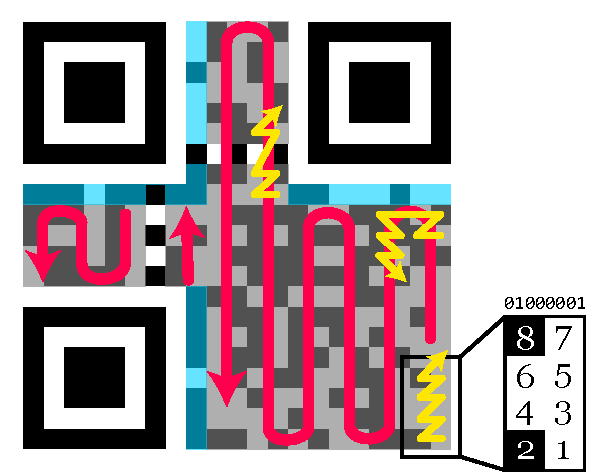
\includegraphics[width=0.6\linewidth]{zigzag.pdf}
\caption{Opbouw QR-code}
\label{fig:zigzag}
\end{figure}
De bits kunnen nu in de QR-code geplaatst worden. Dat gebeurt met een dubbel zigzag-patroon. Er wordt rechts-onder begonnen, in de hoek zonder finder-pattern. Een 1 wordt een zwarte module en een 0 een witte module. Modules zijn de vierkante blokjes waaruit QR-codes zijn opgebouwd.

Figuur \ref{fig:zigzag} laat de plaatsing van de bits zien. Bij de blauwe gebieden moet plaats worden vrijgehouden voor de `format string', die we later toevoegen. De pijlen in de afbeelding geven de volgorde aan waarin de bits in de QR-code gezet moeten worden. Dit waren de bits die we het vorige hoofdstuk hebben berekend:\\\\
\blockms{01000001 00000100 00110110 11110110 01000110 01010111 00100110 10010110 11100110 01110111 00110111 01000110 1000011001010110 11110111 00100110 10010110 01010000 1110110010001000 11100010 10000011 01011000 01010101 11010001 11011010\\}
De eerste bit is een 0, dus in de QR-code wordt rechtsonder een witte module getekend. Daarna komt een 1, dus een zwarte module. Schuin daarboven wordt weer een witte module getekend, en ga zo maar door. Als je bovenaan bent gekomen, ga je in de volgende kolom weer omlaag.

Kom je de timing-pattern tegen (de stippellijntjes), sla je die over en zoek je de eerstvolgende lege plek. In grotere QR-code's moet je ook nog rekening houden met de `aligment pattern'  rechtsonder. Net als bij de timing-pattern sla je dan de gebruikte modules over tot je weer een lege plek tegenkomt, dan ga je weer verder.

Niet bij alle QR-code versies komt het aantal bits mooi uit. Er blijven dan achteraan een paar lege modules over. Die mogen wit blijven, maar moeten wel gemaskt worden, net als de rest.

\subsubsection{`Masking'}
\begin{figure}[!htbp]
\centering
\includegraphics[width=0.8\linewidth]{mask-patterns.png}
\caption[Mask-patterns]{Maks-patterns\footnotemark}
\label{fig:mask-patterns}
\end{figure}
\footnotetext{Afbeelding uit QR-code specificaties (ISO/IEC 18004 blz. 49)}

\begin{wrapfigure}[13]{r}{0.2\linewidth}
\includegraphics[width=\linewidth]{waarom-masks.png}
\caption{Masking voorkomt zulke codes}
\label{fig:waarom-mask}
\end{wrapfigure}
\begin{figure}[!htbp]
\centering
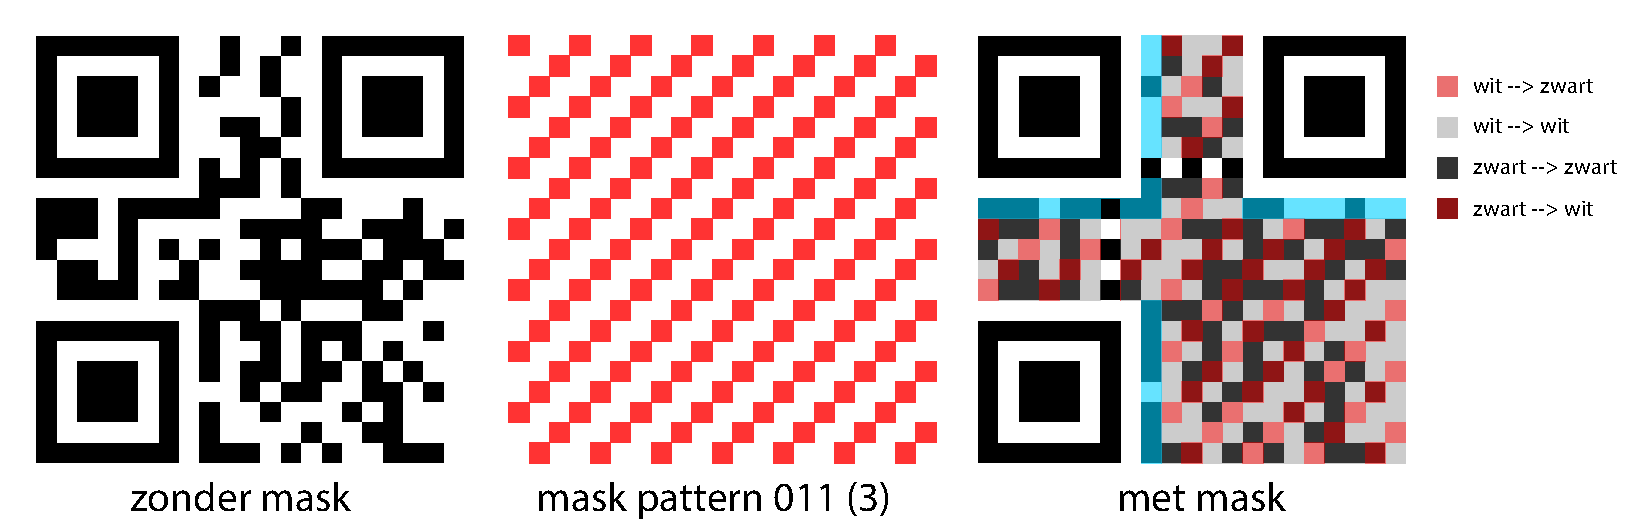
\includegraphics[width=\linewidth]{mask-qr.pdf}
\caption{mask-pattern 011 toepassen}
\label{fig:apply-mask}
\end{figure}

De volgende stap is een `mask' toepassen, zodat de QR-code beter te scannen wordt. Als er toevallig in de QR-code ergens een finding-pattern ontstaat, zou de scanner van slag kunnen raken, zoals in Figuur \ref{fig:waarom-mask}. Om dat op te lossen moeten er verschillende patronen `overheen gelegd' worden, en wordt gekozen welke code het best te scannen is. Hoe die keuze wordt gemaakt, behandel ik later.

Figuur \ref{fig:mask-patterns} laat de acht verschillende patronen zien die gebruikt kunnen worden. Elk patroon wordt gevormd door een bepaalde functie met als argumenten de coördinaten. In de functies wordt modulo 2 of 3 gerekend, waardoor het patroon zich herhaalt. De finder-patterns, de format-string en de alignment-pattern worden niet veranderd door de mask, alleen de inhoud van de QR-code. Is de functie gelijk aan nul op een bepaalde positie, dan moet de de kleur van van de module worden omgedraaid. In Figuur \ref{fig:apply-mask} is te zien hoe mask-pattern 011 kan worden toegepast op onze QR-code.

Ik heb een functie geprogrammeerd die de QR-code vult, en meteen een mask toepast. Het algoritme om de QR-code te vullen is best ingewikkeld, en het was moeilijk om te maken. De zessen die je ziet hebben te maken met het feit dat er in de zesde kolom een kolom wordt overgeslagen vanwege de linker timing-pattern.
\begin{minted}[fontsize=\small]{python}
class Qr_code:
    ...
    def vul_qr_code(self,qr_bits):
        '''vul de qr-code met bits'''
        # masking formules
        masking = {
            # modulo wordt geschreven als %
            0 : (lambda x,y: (x+y)%2),
            1 : (lambda x,y: y%2),
            2 : (lambda x,y: x%3),
            3 : (lambda x,y: (x+y)%3),
            4 : (lambda x,y: (y/2 + x/3)%2),
            5 : (lambda x,y: (x*y)%2+(x*y)%3),
            6 : (lambda x,y: ((x*y) % 2 + (x*y) % 3) % 2),
            7 : (lambda x,y: ((x*y) % 3 + (x+y) % 2) % 2)
            }
        class vector(list):
            ''' Vectoren kunnen worden opgeteld: vector(3,-1) += (1,2) --> (4,1) '''
            def __iadd__(self,other):
                    return self.__class__([self[0]+other[0],self[1]+other[1]])
        g = self.grootte
        # De positie waar wordt begonnen is rechtsonder
        pos = vector([g-1,g-1])
        # Bij de laatste bit moet worden gestopt
        last_bit = len(qr_bits)-1
        for i,bit in enumerate(qr_bits):
            # stel de mask-formule gelijk aan 0
            mask = int(masking[self.mask](pos[0],pos[1]) == 0)
            # verwissel een 1 met een 0 als de vergelijking waar is
            self.matrix[tuple(pos)] = str( mask ^ int(bit) )
            # stop bij de laatste bit
            if i==last_bit:
                break
            # sla de linker timing-pattern over
            if tuple(pos) == (7,9):
                pos += (-2,0)
                continue
            # algoritme voor het zigzag-patroon
            while True:
                dir = 'up'
                if pos[0] < 6 and pos[0] % 4 < 2:
                    dir = 'down'
                if pos[0] > 6 and (pos[0]-1) % 4 < 2:
                    dir = 'down'
                if (pos[0]%2 and pos[0]<6) or (not pos[0]%2 and pos[0]>6):
                    pos += (-1,0)
                # einde van de kolom
                elif (dir=='up' and pos[1]==0) or (dir=='down' and pos[1]==g-1):
                    pos += (-1,0)
                else:
                    pos += (1,(-1 if dir=='up' else 1))
                if self.matrix[tuple(pos)] == -1:
                    # als de module leeg is, zoek dan niet verder
                    break
        # maak overige pixels wit
        for i in range(0,g):
            for j in range(0,g):
                if self.matrix[(i,j)] == -1:
                    self.matrix[(i,j)] = 0 if masking[self.mask](i,j) else 1
\end{minted}

\subsubsection{`Format information'}
\begin{figure}[htbp]
\centering
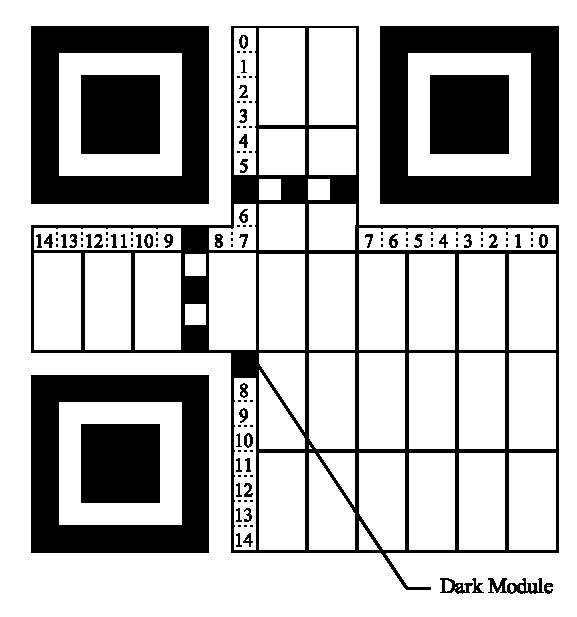
\includegraphics[width=0.4\linewidth]{format-string.pdf}
\caption[Format information]{Format information\footnotemark}
\label{fig:format-string}
\end{figure}
\footnotetext{Afbeelding uit QR-code specificaties (ISO/IEC 18004 blz. 54)}
Als laatste moet de format-string worden toegevoegd, die de gebruikte mask en het e.c-level bevat. Deze informatie is met een eenvoudige RS-code gecodeert, en twee keer in de QR-code opgeslagen rondom de drie finder-patterns. Zo weet de scanner welke mask op de QR-code is toegepast en met welk e.c.-level gedecodeerd kan worden.

Deze format-string is bestaat uit 15 bits, die worden geplaatst rondom de finder-patterns, zoals in figuur \ref{fig:format-string}. Er is ook te zien waar de `dark-module' wordt geplaatst, deze module is altijd zwart volgens de QR-code specificaties en maakt geen deel uit van de format-string.

De eerste twee bits geven het e.c-level aan. In de tabel hieronder is te zien welke bits je moet toevoegen. We zijn een 1-L code aan het coderen, dus de format-string begint met \texttt{01}. Daarna wordt het nummer van de gebruikte mask in drie bits toegevoegd. Als we bijvoorbeeld mask-3 gebruiken, wordt dat binair \texttt{011}. Samengevoegd wordt dat dan \texttt{01011}.

\[
\setlength{\tabcolsep}{10pt}
\def\arraystretch{1.5}
\begin{tabular}{|c|c|}
\hline
\bfseries E.C-level & \bfseries Bits\\\hline
L & \texttt{01}\\\hline
M & \texttt{00}\\\hline
Q & \texttt{11}\\\hline
H & \texttt{10}\\\hline
\end{tabular}
\]

Nu moeten deze bits worden gecodeerd met een simpele variant van de Reed-Solomoncode. Deze codering werkt in een simpel lichaam: $\{0,1\}$, dus reken gaat per bit. De rekenregels zijn erg logisch:
$$0 \xor 0=0$$
$$0 \xor 1=1$$
$$1 \xor 1=0$$
$$0\cdot0=0$$
$$1\cdot0=0$$
$$1\cdot1=1$$

De bits worden geschreven als een polynoom en gedeeld door de generatorpolynoom, waarbij de laagste macht van $x$ het aantal e.c-codewoorden is (de lengte van de generatorpolynoom - 1).
$$\frac{0x^{14}+1x^{13}+0x^{12}+1x^{11}+1x^{10}}
{1x^{10}+0x^9+1x^8+0x^7+0x^6+1x^5+1x^4+0x^3+1x^2+1x^1+1}
$$

We gebruiken hier ook een syntetische deling om de redundantie te berekenen:

\[
\setlength{\tabcolsep}{2pt}
\begin{tabular}{rrrrrrrrrr|rrrrrrrrrrrrrrr}
&&&&&&&&&&0&1&0&1&1&0&0&0&0&0&0&0&0&0&0\\
&&&&&&&&&1&&&&&&&&&&&&1&&&1\\
&&&&&&&&1&&&&&&&&&&&&1&&&1&\\
&&&&&&&1&&&&&&&&&&&&1&&&1&&\\
&&&&&&0&&&&&&&&&&&&&&&&&&\\
&&&&&1&&&&&&&&&&&&1&&&1&&&&\\
&&&&1&&&&&&&&&&&&1&&&1&&&&&\\
&&&0&&&&&&&&&&&&&&&&&&&&&\\
&&0&&&&&&&&&&&&&&&&&&&&&&\\
&1&&&&&&&&&&&&1&&&1&&&&&&&&\\
0&&&&&&&&&&&&&&&&&&&&&&&&\\\cline{11-25}
&&&&&&&&&&0&1&0&0&\multicolumn{1}{r|}{1}&0&0&1&0&0&0&1&1&1&1
\end{tabular}
\]

De rest is \texttt{0010001111}. De rest wordt toegevoegd aan de data-bits, dus de gecodeerde format-string is \texttt{010110010001111}. Dat moet met nog geXORed worden volgens de QR-code specificaties. Dit is om te voorkomen dat de format-string bij een bepaalde versie alleen uit nullen zou bestaat, en dat zou moeilijk te scannen zijn.

\blockms{\\
010110010001111\\
101010000010010\\
----------------- XOR\\
111100010011101\\}

Nu worden deze bytes van achter naar voren in de QR-code geplaatst. De eerste bit moet dus bij 14 worden ingevuld, de tweede bij 13 en de laatste bit bij 0, zoals in Figuur \ref{fig:format-string} staat aangegeven. Deze stappen heb ik weer geprogrammeerd:
\begin{minted}[fontsize=\small]{python}
class Qr_code:
    ...
    def voeg_format_string_toe(self):
        # Error-Correction Level
        ec_indicator = {
            'L' : '01',
            'M' : '00',
            'Q' : '11',
            'H' : '10',
        }
        format_string = ec_indicator[self.ec]+"{0:03b}".format(self.mask)
        # Binaire Synthetische Deling
        teller = output = [int(x) for x in list(format_string)] + [0]*10
        # noemer is generatorpolynoom:
        noemer = [1,0,1,0,0,1,1,0,1,1,1]
        # Voor alle diagonalen die passen
        for i in range(0, len(teller) - (len(noemer)-1)):
            if output[i] != 0: # log(0) bestaat niet
                # de eerste coöficiënt van de noemer wordt overgeslagen
                for j in range(1, len(noemer)):
                    if noemer[j] != 0: # log(0) bestaat niet
                        output[i+j] ^= 1 # 1*1=1
        separator = -(len(noemer)-1)
        rest = output[separator:]
        format_string = format_string + ''.join([str(x) for x in rest])
        # zet om naar een nummer voor de masking
        format_string = int(format_string,2)
        # mask met Exclusive OR
        format_string ^= 21522
        # zet weer om naar bits
        format_string = "{0:015b}".format(format_string)
        s = self.grootte
        # posities rondom de `finder patterns'
        format_pos = {
            (8,0):0,
            (8,1):1,
            (8,2):2,
            ...
            (8,s-2):13,
            (8,s-1):14
        }
        for pos,i in format_pos.items():
            self.matrix[pos] = format_string[14-i]
        # voeg `dark module' toe
        self.matrix[(8,s-8)] = 1
\end{minted}

\subsubsection{Mask kiezen}
\begin{figure}[htbp]
\centering
\includegraphics[width=0.9\linewidth]{masks.png}
\caption{QR-code van het woord `Coderingstheorie' maar met verschillende masks}
\label{fig:masks}
\end{figure}
Nu kan het programma een volledige QR-code maken! Met dit commando bouw je een QR-code met de tekst `Coderingstheorie', met e.c-level Low en mask 011 (3):

\begin{minted}[fontsize=\small]{python}
Qr_code('Coderingstheorie', ec='L', mask=3)
\end{minted}

In Figuur \ref{fig:masks} is dezelfde QR-code met alle acht masks getoond. Er zijn vier regels die punten aftrek geven, en de code met de minste punten wordt gekozen.
\begin{enumerate}
    \item Als er meer dan vier modules met dezelfde kleur op een rij staan, horizontaal of verticaal. Voor de eerste vijf worden drie punten afgetrokken en voor iedere module meer één punt extra.
    \item Drie punten aftrek voor elk blokje van twee bij twee modules van dezelfde kleur.
    \item Veertig punten voor elke keer dat het patroon 1011101 met vier nullen ervoor of erachter voorkomt, horizontaal of verticaal. Dit patroon lijkt namelijk op de finder-pattern, en moet worden voorkomen.
    
    Bijvoorbeeld: \includegraphics[scale=.8]{pattern-1011101.png}
    \item De verhouding van licht en donker moet zo gelijk mogelijk zijn. Het aantal punten wordt zo berekend:
    \begin{minted}[fontsize=\small]{python}
    # Bereken het percentage dat het aantal zwarte modules afwijkt van 50%
    ratio = black_modules / total_modules
    percent = (ratio * 100) - 50
    # Bereken de absolute waarde, deel door vijf, rond af en vermenigvuldig met 10
    aantal_punten = int(abs(percent)/5)*10
    \end{minted}
\end{enumerate}
Als we van alle codes nu de score berekenen, komen we op deze getallen: 421, 360, 431, 386, 393, 483, 479 en 296 (respectievelijk van mask 0 tot mask 7). Omdat mask 7 het minste strafpunten heeft, kunnen we die het best gebruiken.
\subsection{Hoe werkt het decoderen?}
Het scannen van een QR-code, is ook een ingewikkeld proces. Veel scanners voor QR-codes maken continu foto's en zoeken daarin naar de drie finder-patterns. Als die zijn gevonden, wordt met behulp van de timing-patterns (de stippellijntjes) de grootte bepaald van de QR-code. De format-information rondom de finder-patterns wordt dan gedecodeerd, om de e.c-level en de mask uit te lezen.

Dan wordt de mask van de QR-code gehaald, en worden de modules in het zigzag-patroon op de juiste volgorde gezet. De software zet de modules om in bits en verdeelt die in bytes (8 bits). Die bytes vormen de codewoorden die met de Reed-Solomoncode zijn gecodeerd. Nu moet er worden gecontroleerd of de QR-code foutloos is gescand, en daarvoor is wiskunde nodig:

$$ \frac{10^n \cdot msg_{in}(x)}{g_n(x)}=\text{quotiënt}+\frac{\text{rest}}{g_n(x)}$$
$$ msg_{out}(x) = 10^n \cdot msg_{in}(x) - \text{rest} $$

In deze vergelijkingen is $n$ het aantal e.c-codewoorden, $g_n(x)$ de generatorpolynoom, $msg_{in}$ de polynoom van het te coderen bericht en $msg_{out}$ het gecodeerde bericht. Merk op dat $msg_{out}(x)$ deelbaar is door $g_n(x)$. Om dat te zien, kan je een getallenvoorbeeld gebruiken:

$$ \frac{7}{3} = 2 + \frac{1}{3} $$
$$ 7 - 1 = 0 \mod{6} $$

Als van $msg_{out}(x)$ de rest wordt afgetrokken, is het dus deelbaar door de generatorpolynoom. Dat betekent dat de oplossingen van $g_n(x)=0$ element zijn van de oplossingen van $msg_{out}(x)=0$, dus $msg_{out}(x)$ heeft nulpunten op dezelfde plaatsen als de generatorpolynoom. De nulpunten van $g_n(x)$ zijn makkelijk af te leiden uit de definitie:

$$g_n(x)=\prod\limits_{i=0}^{n-1} x-\alpha^i = (x-\alpha^0)(x-\alpha^1)(x-\alpha^2) ... (x-\alpha^{n-1})=0$$
$$x=\alpha^0 \lor x=\alpha^1 \lor x=\alpha^2 \lor (...) \lor x=\alpha^{n-1}$$

De eerste stap van het decoderen is controleren of de QR-code foutloos is gescand, wat wordt gedaan door de `syndromes polynomial' te berekenen. Zo wordt gecontroleerd of $msg_{out}$ inderdaad nulpunten heeft bij $\alpha^0$ tot $\alpha^{n-1}$. De syndromes-polynoom heeft deze definitie:
$$ synd(x) = \sum\limits_{i=0}^{n-1} msg(\alpha^{n-i-1})\cdot x^{i}$$
$$ synd(x) = msg(\alpha^0)\cdot x^{n-1} + msg(\alpha^1)\cdot x^{n-2} + (...) + msg(\alpha^n-1)\cdot x^{0} $$

Wanneer alle termen van de syndromes-polynoom gelijk zijn aan 0, bevat de gescande QR-code geen fouten. Zijn er wel fouten, dan kunnen algoritmes zoals het Forney algoritme en het Berlekamp–Massey algoritme de fouten lokaliseren en verbeteren. Deze algoritmes maken gebruik van de syndromes-polynoom, die alle informatie bevat om fouten te herstellen.

Nadat eventuele fouten zijn verwijdert, leest de software de mode-indicator en de lengte van het bericht. Daarna kunnen de bytes worden omgezet naar letters. Het bericht in de QR-code kan dan worden getoond op het scherm. Als het een adres is van een website, wordt de link vaak direct geopend in een browser.

\section{Conclusie}
Vorig schooljaar heb ik de reader `Foutje? Dat verbeteren we toch!' van de TU/e doorgewerkt, en daarin werd een eenvoudige RS-code uitgelegd. Toen ik na de zomervakantie de codering van QR-codes ging bestuderen, bleek de RS-code daar veel ingewikkelder te zijn. Ik las eerst een artikel dat wel de stappen liet zien voor het coderen, maar niet uitlegde waarom. Het heeft even geduurd voordat ik een duidelijke uitleg vond over de RS-code die in QR-codes wordt gebruikt. Ik heb vaak gedacht: Nu snap ik het helemaal. Maar daar moest ik dan op terugkomen. Ik begreep het pas echt toen ik het programma aan het schrijven was.

Als ik zoiets opnieuw zou doen, dan maak ik eerst een plan wat er allemaal in het programma moet komen. Nu had ik eerst een programma gemaakt dat alleen grootte drie kon maken. Later breidde ik dat uit met grootte één tot vier, waardoor ik veel code weer moest aanpassen. Daarna liet ik het programma ook nog grootte vijf en zes ondersteunen, en moest ik weer veel opnieuw programmeren. Het was veel efficiënter geweest om het in een keer goed te doen. Ik heb dus geleerd om eerst een plan te maken voor een programma, en dan pas te beginnen. 

Het maken van het werkstuk was helemaal niet eentonig. Er zat wiskunde in, ik kon programmeren en over de geschiedenis schrijven. Ook heb ik de meeste afbeeldingen zelf gemaakt, wat best wat tijd kostte.

Het was een hele uitdaging om me in dit onderwerp te verdiepen, maar het is me uiteindelijk goed gelukt om de hoofdvraag te beantwoorden. Ik heb zelf een programma geschreven, en dus eigenlijk aan de computer uitgelegd hoe een QR-code werkt. Als je iets duidelijk kan uitleggen, begrijp je het pas echt goed. Daarom heb ik er ook voor gekozen mijn werkstuk zo aan te pakken.

Deze aanpak heeft ook mijn ervaring met programmeren vergroot, en dat helpt ook bij mijn studiekeuze. Door dit project ben ik erachter dat programmeren echt mijn ding is, en heb ik besloten informatica te gaan studeren.

\newpage
\section{Bronvermelding}
\begin{itemize}
\item Officiële QR-code specificaties (ISO/IEC CD 18004)
\item \url{http://www.matchadesign.com/news/blog/qr-code-demystified-part-1/}
\item \url{http://www.thonky.com/qr-code-tutorial/}
\item \url{https://en.wikiversity.org/wiki/Reed-Solomon_codes_for_coders}
\item \url{https://plus.maths.org/content/os/issue3/codes/index}
\item \url{http://www.win.tue.nl/~jessers/aansluiting/foutje.pdf}
\item \url{http://bloch.ece.gatech.edu/sp10_ece6606/coding_history.pdf}
\item \url{https://en.wikipedia.org/wiki/BCH_code}
\item \url{https://nl.wikipedia.org/wiki/BCH-code_(coderingstheorie)}
\item \url{https://nl.wikipedia.org/wiki/Hamming-code}
\item \url{https://en.wikipedia.org/wiki/Synthetic_division}
\item \url{https://nl.wikipedia.org/wiki/Wet_van_Shannon-Hartley}
\item \url{https://en.wikipedia.org/wiki/Low-density_parity-check_code}
\item \url{https://en.wikipedia.org/wiki/QR_code}
\end{itemize}

\end{document}